\chapter{Conception de la solution}
\label{chap:conception}

Ce chapitre passe du diagnostic à la conception. Il part des besoins recueillis sur le terrain (section~\ref{chap:besoins}), les traduit en modèles UML (section~\ref{chap:modelisation}), puis fixe l'architecture logicielle en vues C4 et en décisions tracées (section~\ref{chap:architecture}).

\section{Analyse des besoins}
\label{chap:besoins}
L'analyse des besoins fait le lien entre le diagnostic du chapitre~\ref{chap:contexte} et la conception qui suit. Elle pose un cahier des charges clair et vérifiable, qui guide les choix de conception de l'architecture hybride : ce que le système doit faire, et avec quelle qualité. Les choix technologiques, eux, sont justifiés plus loin.

\subsection{Démarche d'analyse et recueil des besoins}
\label{sec:recueil}
Cette spécification s'appuie sur une démarche d'ingénierie des exigences (\textit{requirements engineering}) qualitative, que nous avons menée au bureau de Dakar. Quatre sources d'information l'alimentent :

\begin{enumerate}
    \item \textbf{L'observation participante} des processus quotidiens au bureau de Dakar, pour voir les pratiques réelles au-delà des procédures déclarées ;
    \item \textbf{L'analyse des documents} produits par l'entreprise (fichiers \texttt{RECAP-*}, fiches d'autorisation de dépenses \texttt{AUT-DEP}), qui révèle la structure implicite des données métier ;
    \item \textbf{Les entretiens semi-directifs} avec les acteurs clés (agent de saisie, assistant principal, chef de bureau, chef logistique), pour recueillir leurs objectifs et leurs frustrations ;
    \item \textbf{L'analyse rétrospective} de seize mois de données historiques (4\,755 transactions, 319 camions, 727 bons de chargement), qui donne la volumétrie réelle à traiter.
\end{enumerate}

Nous formalisons les besoins en exigences numérotées et priorisées, réparties en deux catégories : les \emph{exigences fonctionnelles} (\texttt{EF}) décrivent les services rendus par le système, les \emph{exigences non fonctionnelles} (\texttt{ENF}) en encadrent la qualité avec des métriques chiffrées et vérifiables. Nous priorisons chaque exigence selon \textbf{MoSCoW} (\textit{Must have} : indispensable, \textit{Should have} : souhaitable, \textit{Could have} : optionnel, \textit{Won't have} : hors périmètre), et la rattachons en fin de chapitre aux limites du chapitre~\ref{chap:contexte} et aux hypothèses H1 à~H4.

Cette analyse confirme et prolonge le diagnostic du chapitre~\ref{chap:contexte} (\S1.3.3) : ses quatre catégories de limites (opérationnelles, qualitatives, décisionnelles, stratégiques) restent le point d'ancrage des exigences qui suivent. Notre présence sur le terrain a surtout précisé trois choses concrètes. La redondance de saisie entre le cahier manuscrit de l'Assistant Principal et le tableur de l'Agent de Saisie génère des doublons différés, difficiles à détecter. Le circuit de validation par signatures manuscrites ajoute de la latence. Et le suivi de caisse reste opaque : l'Assistant Principal n'a aucun accès autonome au solde disponible. L'analyse de l'existant a aussi permis de cerner le périmètre de \texttt{kiri.app}, déjà en usage : cantonnée à la conformité administrative (pièces signées par les représentants logistiques), elle n'a aucun module analytique ou décisionnel.

\subsection{Parties prenantes et personas}
\label{sec:personas}
Concevoir une plateforme alignée sur le terrain suppose de savoir \emph{qui} va l'utiliser, et \emph{pourquoi}. On distingue trois catégories de parties prenantes. Les \textbf{utilisateurs directs} (Agent de Saisie, Assistant Principal, Chef de Bureau, Chef Logistique, Administrateur Système) manipulent l'application au quotidien. Les \textbf{utilisateurs indirects} en profitent sans l'utiliser eux-mêmes, au premier rang desquels la direction de SOYAFF à Bamako, qui reçoit le reporting consolidé. Les \textbf{parties prenantes contextuelles}, elles, n'utilisent jamais le système mais pèsent sur sa conception : la réglementation sénégalaise sur la protection des données (loi 2008-12), les autorités douanières, les tutelles communautaires (UEMOA, CEDEAO).

Nous avons caractérisé cinq profils d'utilisateurs directs (P1 à~P5) selon leur rôle, leur localisation et leur maturité numérique. Côté applicatif, ces cinq personas se rattachent à trois rôles RBAC (cf. ENF-SEC-03) : P1, P2 et P3, tous basés à Dakar, partagent le rôle \texttt{DAKAR\_AGENT} avec des périmètres fonctionnels distincts ; P4 porte le rôle \texttt{BAMAKO\_CHEF} ; P5 porte le rôle \texttt{ADMIN}. Ce mapping (dernière colonne du tableau~\ref{tab:cartographie_acteurs}) structurera les acteurs des diagrammes de cas d'utilisation de la section suivante.

\begin{table}[htbp]
\centering
\footnotesize
\caption{Cartographie des acteurs et profils numériques du corridor SOYAFF}
\label{tab:cartographie_acteurs}
\begin{tabularx}{\linewidth}{|>{\raggedright\arraybackslash}p{0.8cm}|>{\raggedright\arraybackslash}X|>{\raggedright\arraybackslash}X|>{\raggedright\arraybackslash}p{2.0cm}|>{\raggedright\arraybackslash}X|>{\raggedright\arraybackslash}p{2.3cm}|}
\hline
\rowcolor[HTML]{EFEFEF}
\textbf{ID} & \textbf{Acteur / Fonction} & \textbf{Rôle Opérationnel} & \textbf{Localisation} & \textbf{Maturité Numérique} & \textbf{Rôle RBAC} \\ \hline
\textbf{P1} & Agent de Saisie & Saisie des dépenses, édition des récaps journaliers. & Dakar & Intermédiaire (maîtrise d'Excel et de WhatsApp). & \texttt{DAKAR\_AGENT} \\ \hline
\textbf{P2} & Assistant Principal & Gestion directe de la caisse, supervision de premier niveau. & Dakar & Basique (pratique exclusive des supports physiques). & \texttt{DAKAR\_AGENT} \\ \hline
\textbf{P3} & Chef de Bureau & Validation finale des opérations, supervision générale. & Dakar & Basique (validation par signature manuscrite). & \texttt{DAKAR\_AGENT} \\ \hline
\textbf{P4} & Chef Logistique & Arbitrage, décision stratégique, reporting financier. & Bamako & Orienté reporting (consommateur de KPIs et d'analyses). & \texttt{BAMAKO\_CHEF} \\ \hline
\textbf{P5} & Administra\-teur Système & Conception, déploiement et maintenance de la solution. & Dakar (déporté) & Spécialisé en génie logiciel. & \texttt{ADMIN} \\ \hline
\end{tabularx}
\end{table}

Chaque profil fait face à des contraintes spécifiques qui dictent les exigences fonctionnelles de la future plateforme :

\begin{enumerate}
    \item \textbf{P1, l'Agent de Saisie (Dakar) :} sa frustration vient de la double saisie (cahier manuscrit vers Excel) et de la lenteur des signatures physiques du Chef de Bureau et de l'Assistant Principal. Il ne peut pas non plus requêter rapidement l'historique des dépenses pour répondre à sa hiérarchie.
    \item \textbf{P2, l'Assistant Principal (Dakar) :} responsable de la caisse, il a besoin de connaître en temps réel le solde disponible (approvisionnements de Bamako moins dépenses locales). Sans outil de synchronisation, il dépend du poste de l'agent de saisie pour suivre ses flux financiers.
    \item \textbf{P3, le Chef de Bureau (Dakar) :} son rôle se limite à valider des documents imprimés. Son passage au numérique doit rester simple, vu sa maîtrise informatique basique.
    \item \textbf{P4, le Chef Logistique (Bamako) :} le plus touché par les défaillances actuelles, il loue une flotte de \textit{camions particuliers} en plus de la flotte SOYAFF. Il gère à la main un double flux financier : une \textbf{avance} au départ, un \textbf{reliquat} au déchargement à Bamako (ou géré par Dakar si le camion s'arrête à la frontière). Sans automatisation, il doit tout ressaisir pour avoir la moindre visibilité.
    \item \textbf{P5, l'Administrateur Système (Dakar, déporté) :} garant de la disponibilité et de la sécurité de la plateforme, il a besoin de gérer les comptes et les rôles, de consulter les journaux d'audit et de superviser l'état des services (ETL, RAG, application web). Sa préoccupation : garder la solution opérationnelle et souveraine avec peu de ressources.
\end{enumerate}

Cette diversité de profils, du terrain à maturité numérique basique jusqu'à l'administrateur technique, impose une plateforme multi-rôles avec un contrôle d'accès finement différencié.

\subsection{Besoins fonctionnels}
\label{sec:besoins_fonctionnels}
Nous organisons les besoins fonctionnels en six modules : ingestion et saisie (\texttt{EF-ETL} / \texttt{EF-SDR}), validation hiérarchique (\texttt{EF-VAL}), consolidation et reporting (\texttt{EF-REP}), tableau de bord décisionnel (\texttt{EF-DSH}), module conversationnel hybride (\texttt{EF-RAG}), administration (\texttt{EF-ADM}). Chaque exigence est rattachée à un ou plusieurs personas, priorisée par MoSCoW et tracée vers la limite du chapitre~\ref{chap:contexte} (\S1.3.3) dont elle vient.

\begin{longtable}{|>{\raggedright\arraybackslash}p{1.5cm}|>{\raggedright\arraybackslash}p{5.2cm}|>{\raggedright\arraybackslash}p{1.6cm}|>{\raggedright\arraybackslash}p{1.7cm}|>{\raggedright\arraybackslash}p{2.8cm}|}
\caption{Matrice de spécification des exigences fonctionnelles (SOYAFF)}
\label{tab:exigences_fonctionnelles} \\
\hline
\rowcolor[HTML]{EFEFEF}
\textbf{ID} & \textbf{Description de l'exigence fonctionnelle} & \textbf{Persona} & \textbf{Priorité} & \textbf{Origine (\S1.3.3)} \\ \hline
\endfirsthead

\multicolumn{5}{c}{\tablename\ \thetable\ -- suite de la page précédente} \\
\hline
\rowcolor[HTML]{EFEFEF}
\textbf{ID} & \textbf{Description de l'exigence fonctionnelle} & \textbf{Persona} & \textbf{Priorité} & \textbf{Origine (\S1.3.3)} \\ \hline
\endhead

\hline
\multicolumn{5}{r}{\textit{Suite page suivante}} \\
\endfoot

\hline
\endlastfoot

\multicolumn{5}{|l|}{\cellcolor[HTML]{DDEBF7}\textbf{M1. Ingestion et saisie unifiée des données}} \\ \hline
\textbf{EF-ETL-01} & \textbf{Importation des données historiques :} le système doit permettre l'importation des fichiers tableurs (Excel) de suivi opérationnel existants. & P1, P2 & Must & Opérationnelle \\ \hline
\textbf{EF-ETL-02} & \textbf{Détection des doublons temporels :} lors de l'importation ou de la saisie, le système doit repérer une dépense potentiellement dupliquée sur une fenêtre temporelle configurable, émettre une alerte et exiger une confirmation explicite de l'opérateur avant enregistrement. & Système, P2 & Must & Qualitative \\ \hline
\textbf{EF-SDR-01} & \textbf{Saisie directe via formulaires :} le système doit fournir des formulaires d'insertion directe centralisant la logique métier, afin de remplacer progressivement les fichiers Excel. & P1 & Should & Opérationnelle \\ \hline
\textbf{EF-SDR-02} & \textbf{Contrôle métier des rations :} le système doit contrôler l'intervalle entre deux rations octroyées à un même chauffeur. En deçà de deux jours, l'octroi est bloqué (rejet automatique) ; entre deux et cinq jours, une alerte est levée et une confirmation explicite de l'opérateur est exigée avant enregistrement. & Système & Must & Qualitative \\ \hline
\textbf{EF-SDR-03} & \textbf{Journalisation de l'historique :} le système doit conserver et rendre consultable l'intégralité de l'historique des opérations, levant la crainte de perte de données exprimée par P1. & P1, P2 & Must & Opérationnelle \\ \hline

\multicolumn{5}{|l|}{\cellcolor[HTML]{DDEBF7}\textbf{M2. Validation hiérarchique}} \\ \hline
\textbf{EF-VAL-01} & \textbf{Traçabilité de la validation :} le système doit consigner l'état de validation de chaque transaction. Dans le périmètre du présent mémoire, le circuit s'appuie sur les visas papier existants, dont la référence est enregistrée. & P2, P3 & Must & Opérationnelle \\ \hline
\textbf{EF-VAL-02} & \textbf{Workflow de validation numérique :} le système devrait offrir un circuit de validation dématérialisé (soumission, approbation ou rejet motivé, notification des acteurs) remplaçant les signatures manuscrites. & P1, P2, P3 & Should & Opérationnelle \\ \hline

\multicolumn{5}{|l|}{\cellcolor[HTML]{DDEBF7}\textbf{M3. Consolidation et reporting}} \\ \hline
\textbf{EF-REP-01} & \textbf{Génération automatique du récapitulatif journalier :} le système doit produire automatiquement le récapitulatif journalier, remplaçant le fichier \texttt{RECAP-JOURNALIERE}. & P1, P4 & Must & Opérationnelle \\ \hline
\textbf{EF-REP-02} & \textbf{Consolidation mensuelle :} le système doit générer le récapitulatif mensuel consolidé, supprimant la ressaisie effectuée à Bamako. & P4 & Must & Décisionnelle \\ \hline
\textbf{EF-REP-03} & \textbf{Export des rapports :} le système doit permettre l'export des récapitulatifs et analyses aux formats PDF et Excel. & P4 & Should & Décisionnelle \\ \hline
\textbf{EF-REP-04} & \textbf{Recherche multi-critères :} le système doit permettre de filtrer et rechercher les opérations selon plusieurs critères (période, camion, chauffeur, catégorie de dépense). & P1, P4 & Should & Qualitative \\ \hline

\multicolumn{5}{|l|}{\cellcolor[HTML]{DDEBF7}\textbf{M4. Tableau de bord décisionnel}} \\ \hline
\textbf{EF-DSH-01} & \textbf{Suivi de caisse en temps réel :} le système doit calculer et restituer instantanément le solde de caisse sur le tableau de bord de l'assistant. & P2 & Must & Décisionnelle \\ \hline
\textbf{EF-DSH-02} & \textbf{Visualisation de la flotte :} le système doit intégrer un onglet « Camions » répertoriant l'ensemble de la flotte logistique connectée. & P4 & Must & Décisionnelle \\ \hline
\textbf{EF-DSH-03} & \textbf{Classification de la flotte :} le système doit catégoriser visiblement les camions par étiquettes distinctives (\texttt{camions\_societe} ou \texttt{particuliers}). & P4 & Should & Décisionnelle \\ \hline
\textbf{EF-DSH-04} & \textbf{Consultation du profil véhicule :} au clic sur un camion, le système doit afficher l'historique de ses dépenses et ses dernières positions géographiques. & P4 & Should & Décisionnelle \\ \hline
\textbf{EF-DSH-05} & \textbf{Signalement des anomalies :} le système devrait détecter et signaler les dépenses hors normes (dérive de coût par camion, montants aberrants). & P4 & Could & Stratégique \\ \hline

\multicolumn{5}{|l|}{\cellcolor[HTML]{DDEBF7}\textbf{M5. Module conversationnel hybride (RAG)}} \\ \hline
\textbf{EF-RAG-01} & \textbf{Interface en langage naturel :} le système doit embarquer un agent conversationnel interprétant des requêtes analytiques formulées en langage naturel (français) sur les données synchronisées. & P4 & Should & Décisionnelle \\ \hline
\textbf{EF-RAG-02} & \textbf{Analyse décisionnelle des reliquats :} l'agent doit calculer automatiquement le montant total des reliquats à payer pour les camions particuliers arrivés à Bamako sur le mois en cours. & P4 & Should & Décisionnelle \\ \hline
\textbf{EF-RAG-03} & \textbf{Routage hybride cloud / local :} le système doit orienter les requêtes selon leur sensibilité : traitement local souverain pour les données confidentielles, service cloud pour les requêtes complexes non sensibles. & Système, P4 & Must & Stratégique \\ \hline
\textbf{EF-RAG-04} & \textbf{Citation des sources :} l'agent doit citer explicitement les sources documentaires ou les enregistrements ayant fondé chaque réponse. & P4 & Should & Décisionnelle \\ \hline
\textbf{EF-RAG-05} & \textbf{Journalisation des requêtes IA :} le système doit journaliser l'ensemble des requêtes adressées aux modules d'IA à des fins d'audit et d'évaluation. & Système, P5 & Should & Stratégique \\ \hline

\multicolumn{5}{|l|}{\cellcolor[HTML]{DDEBF7}\textbf{M6. Administration}} \\ \hline
\textbf{EF-ADM-01} & \textbf{Gestion des utilisateurs et des rôles :} le système doit permettre de créer, modifier et désactiver les comptes et d'affecter les rôles (RBAC). & P5 & Must & Stratégique \\ \hline
\textbf{EF-ADM-02} & \textbf{Consultation des journaux d'audit :} le système doit donner accès aux journaux des actions sensibles et des requêtes IA. & P5 & Should & Stratégique \\ \hline
\textbf{EF-ADM-03} & \textbf{Sauvegarde et restauration :} le système doit permettre la sauvegarde et la restauration de la base de données. & P5 & Must & Stratégique \\ \hline
\textbf{EF-ADM-04} & \textbf{Supervision de l'état des services :} le système doit permettre de superviser l'état de santé des services (ETL, RAG, application web). & P5 & Should & Stratégique \\ \hline
\end{longtable}

La plateforme doit aussi satisfaire des exigences de qualité, présentées ci-après.

\subsection{Besoins non fonctionnels}
\label{sec:besoins_non_fonctionnels}
La plateforme doit aussi tenir des contraintes de qualité : les exigences non fonctionnelles (ENF), qui conditionnent la viabilité de l'architecture hybride dans un corridor Dakar--Bamako au réseau instable et aux ressources limitées. Nous les organisons en sept catégories (performance, disponibilité et fiabilité, sécurité, souveraineté et conformité, ergonomie, maintenabilité, frugalité), chacune avec une métrique chiffrée, vérifiable au chapitre~\ref{chap:evaluation}.

\begin{longtable}{|>{\raggedright\arraybackslash}p{2.0cm}|>{\raggedright\arraybackslash}p{2.3cm}|>{\raggedright\arraybackslash}p{5.3cm}|>{\raggedright\arraybackslash}p{2.8cm}|}
\caption{Matrice des exigences non fonctionnelles (Qualité et Contraintes)}
\label{tab:exigences_non_fonctionnelles} \\
\hline
\rowcolor[HTML]{EFEFEF}
\textbf{ID} & \textbf{Catégorie} & \textbf{Description de l'exigence} & \textbf{Métrique / Cible} \\ \hline
\endfirsthead

\multicolumn{4}{c}{\tablename\ \thetable\ -- suite de la page précédente} \\
\hline
\rowcolor[HTML]{EFEFEF}
\textbf{ID} & \textbf{Catégorie} & \textbf{Description de l'exigence} & \textbf{Métrique / Cible} \\ \hline
\endhead

\hline
\multicolumn{4}{r}{\textit{Suite page suivante}} \\
\endfoot

\hline
\endlastfoot

\textbf{ENF-PERF-01} & Performance & Le chargement et l'affichage des indicateurs du tableau de bord doivent rester fluides. & $< 5$~s (P95) \\ \hline
\textbf{ENF-PERF-02} & Performance & Le RAG \textbf{cloud} doit restituer l'analyse d'une requête complexe dans un délai maîtrisé. & $< 5$~s (P95) \\ \hline
\textbf{ENF-PERF-03} & Performance & Le RAG \textbf{local souverain} doit restituer une réponse dans un délai tolérable, malgré la contrainte matérielle. & $< 15$~s (P95) \\ \hline
\textbf{ENF-DISP-01} & Disponibilité & L'application de saisie doit intégrer un mode dégradé (hors-ligne) avec mise en cache locale des saisies. & 0 perte de saisie ; resynchro. $< 5$~min après retour réseau \\ \hline
\textbf{ENF-DISP-02} & Disponibilité & Les services critiques doivent garantir une disponibilité opérationnelle mensuelle élevée. & $\geq 99~\%$ / mois \\ \hline
\textbf{ENF-VOL-01} & Volumétrie & Le pipeline ETL doit ingérer le corpus historique existant sans échec ni saturation mémoire. & $\geq 4\,500$ transactions \\ \hline
\textbf{ENF-VOL-02} & Évolutivité & La base de données doit supporter une montée en charge progressive sans refonte structurelle. & $> 50\,000$ lignes / an \\ \hline
\textbf{ENF-SEC-01} & Sécurité & L'authentification des utilisateurs doit être obligatoire et reposer sur des jetons signés. & JWT ; expiration $\leq 24$~h \\ \hline
\textbf{ENF-SEC-02} & Sécurité & Les mots de passe doivent être hachés selon l'état de l'art. & bcrypt, coût $\geq 12$ \\ \hline
\textbf{ENF-SEC-03} & Sécurité & L'accès aux modules doit être cloisonné par contrôle d'accès basé sur les rôles. & RBAC : DAKAR\_AGENT, BAMAKO\_CHEF, ADMIN \\ \hline
\textbf{ENF-SEC-04} & Sécurité & Les actions sensibles doivent être journalisées (piste d'audit). & Audit trail horodaté, 100~\% des actions sensibles \\ \hline
\textbf{ENF-SEC-05} & Sécurité & Toutes les communications réseau doivent être chiffrées. & TLS $\geq 1.2$ \\ \hline
\textbf{ENF-SOUV-01} & Souveraineté & Les données interrogées par l'agent IA local ne doivent transiter vers aucun service tiers externe. & Rétention 100~\% locale \\ \hline
\textbf{ENF-SOUV-02} & Conformité & Le traitement des données personnelles doit respecter le cadre légal sénégalais. & Conformité loi 2008-12 (CDP) \\ \hline
\textbf{ENF-ERG-01} & Ergonomie & L'interface doit être en français et exploitable par des utilisateurs non techniques. & Français ; validation par P1--P4 \\ \hline
\textbf{ENF-ERG-02} & Ergonomie & L'utilisabilité perçue doit atteindre un niveau satisfaisant, mesuré par questionnaire standardisé. & Score SUS $\geq 70/100$ \\ \hline
\textbf{ENF-ERG-03} & Ergonomie & L'interface doit être responsive (poste fixe et mobile) et compatible avec les navigateurs récents. & Chrome, Firefox, Edge (versions récentes) \\ \hline
\textbf{ENF-MAINT-01} & Maintenabilité & L'architecture doit être modulaire, autorisant le remplacement des modèles LLM sans refonte. & Couplage faible ; interface d'inférence abstraite \\ \hline
\textbf{ENF-MAINT-02} & Maintenabilité & Les choix structurants doivent être documentés et le code testé. & ADR par décision majeure ; tests unitaires $\geq 60~\%$ \\ \hline
\textbf{ENF-FRUG-01} & Frugalité & L'infrastructure de déploiement doit rester accessible budgétairement pour une PME subsaharienne (H1). & $< 50$~\texteuro{} / mois \\ \hline
\end{longtable}

Ces besoins, fonctionnels et non fonctionnels, forment le cahier des charges dont voici la synthèse.

\subsection{Synthèse et matrice de traçabilité}
\label{sec:synthese_tracabilite}
Le cahier des charges compte \textbf{25 exigences fonctionnelles} réparties en six modules applicatifs et \textbf{20 exigences non fonctionnelles} réparties en sept catégories de qualité, soit \textbf{45 exigences au total}. Les exigences non fonctionnelles sont transversales, elles contraignent tout le système et ne sont donc pas priorisées individuellement par MoSCoW ; seules les 25 exigences fonctionnelles le sont. Sur ces 25 : \textbf{12 sont \textit{Must have}} (indispensables pour SOYAFF, traitées dans le mémoire), \textbf{12 sont \textit{Should have}} (souhaitables, traitées si le calendrier le permet), et \textbf{1 est \textit{Could have}} (EF-DSH-05, renvoyée aux perspectives). Aucune n'est classée \textit{Won't have}. La dématérialisation complète du circuit de validation (EF-VAL-02), bien que spécifiée, reste priorisée \textit{Should} : le circuit papier existant reste juridiquement valable pendant la transition.

La matrice de traçabilité (Tableau~\ref{tab:matrice_tracabilite}) relie chaque famille d'exigences à l'origine de son besoin terrain (limites du chapitre~\ref{chap:contexte}, \S1.3.3), à l'hypothèse de recherche qu'elle éprouve (H1 à~H4), et aux chapitres de conception et d'évaluation concernés. Chaque exigence part donc d'un problème industriel concret, et sera validée empiriquement.

\begin{longtable}{|>{\raggedright\arraybackslash}p{2.9cm}|>{\raggedright\arraybackslash}p{4.7cm}|>{\centering\arraybackslash}p{1.2cm}|>{\centering\arraybackslash}p{2.0cm}|>{\centering\arraybackslash}p{1.9cm}|}
\caption{Matrice de traçabilité macroscopique du cahier des charges}
\label{tab:matrice_tracabilite} \\
\hline
\rowcolor[HTML]{EFEFEF}
\textbf{Origine du besoin} & \textbf{Exigences associées (EF / ENF)} & \textbf{Hypo\-thèse} & \textbf{Concep\-tion} & \textbf{Évalua\-tion} \\ \hline
\endfirsthead

\multicolumn{5}{c}{\tablename\ \thetable\ -- suite de la page précédente} \\
\hline
\rowcolor[HTML]{EFEFEF}
\textbf{Origine du besoin} & \textbf{Exigences associées (EF / ENF)} & \textbf{Hypo\-thèse} & \textbf{Concep\-tion} & \textbf{Évalua\-tion} \\ \hline
\endhead

\hline
\multicolumn{5}{r}{\textit{Suite page suivante}} \\
\endfoot

\hline
\endlastfoot

\textbf{Opérationnelle} (double saisie, rupture de charge, peur de perte de l'historique) & EF-ETL-01, EF-SDR-01, EF-SDR-03, EF-VAL-01, EF-VAL-02, EF-REP-01, ENF-DISP-01, ENF-VOL-01 & H3 & §~\ref{chap:modelisation}, \ref{chap:architecture}, \ref{chap:etl} & §~\ref{chap:impact_metier} \\ \hline
\textbf{Qualitative} (erreurs, doublons, ruptures de formules) & EF-ETL-02, EF-SDR-02, EF-REP-04, ENF-MAINT-02 & H3 & §~\ref{chap:modelisation}, \ref{chap:etl} & §~\ref{chap:impact_metier} \\ \hline
\textbf{Décisionnelle} (absence de tableau de bord temps réel, opacité de la caisse) & EF-DSH-01 à EF-DSH-04, EF-REP-02, EF-REP-03, EF-RAG-01, EF-RAG-02, EF-RAG-04, ENF-PERF-01, ENF-PERF-02, ENF-PERF-03 & H2, H3 & §~\ref{chap:architecture}, \ref{chap:webapp}, \ref{chap:ia_rag} & §~\ref{chap:benchmark_rag}, \ref{chap:impact_metier} \\ \hline
\textbf{Stratégique} (absence d'historique, dépendance aux personnes clés) & EF-DSH-05, EF-RAG-03, EF-RAG-05, EF-ADM-01 à EF-ADM-04, ENF-VOL-02, ENF-MAINT-01 & H4 & §~\ref{chap:architecture}, \ref{chap:ia_rag} & §~\ref{chap:benchmark_rag}, \ref{chap:generalisation_spl} \\ \hline
\textbf{Souveraineté et infrastructure locale} & EF-RAG-03, ENF-SEC-01 à ENF-SEC-05, ENF-SOUV-01, ENF-SOUV-02 & H2 & §~\ref{chap:architecture}, \ref{chap:ia_rag} & §~\ref{chap:benchmark_rag} \\ \hline
\textbf{Frugalité budgétaire} & ENF-FRUG-01, ENF-DISP-02 & H1 & §~\ref{chap:architecture}, \ref{chap:devops} & §~\ref{chap:impact_metier} \\ \hline
\textbf{Adoption utilisateur} (maturité numérique hétérogène) & ENF-ERG-01, ENF-ERG-02, ENF-ERG-03 & H3 & §~\ref{chap:modelisation}, \ref{chap:webapp} & §~\ref{chap:adoption} \\ \hline
\end{longtable}

Ce cahier des charges fixe le cadre de la conception. Les sections suivantes y répondent : cas d'utilisation en UML, architecture applicative en C4, choix technologiques justifiés chacun par un ADR. Chaque exigence reste reliée à la limite qui la motive et à l'hypothèse qu'elle éprouve, jusqu'à l'évaluation empirique du chapitre~\ref{chap:evaluation}.
\section{Modélisation du système (UML)}
\label{chap:modelisation}

Cette section traduit en modèles UML le cahier des charges formalisé à la section~\ref{chap:besoins}. Il présente successivement la vue statique des acteurs et des fonctionnalités (cas d'utilisation), le modèle de données conceptuel (classes du domaine), les comportements dynamiques des scénarios les plus structurants (séquences) et le circuit de validation hiérarchique (activité). Chaque élément de modélisation est explicitement tracé vers les identifiants d'exigences (\texttt{EF-*}) introduits à la section~\ref{chap:besoins}.

\subsection{Vue des cas d'utilisation}
\label{sec:cas_utilisation}
Les Figures~\ref{fig:cas_utilisation_1} et~\ref{fig:cas_utilisation_2} présentent le diagramme de cas d'utilisation global, scindé en deux vues pour la lisibilité. Les acteurs retenus sont les trois rôles RBAC de \texttt{ENF-SEC-03} (\texttt{DAKAR\_AGENT}, \texttt{BAMAKO\_CHEF}, \texttt{ADMIN}), plus le Planificateur ETL, un acteur non humain porté par Apache Airflow. Les vingt-quatre cas d'utilisation couvrent les exigences fonctionnelles \textit{Must} et \textit{Should} des six modules M1 à M6 ; chaque bulle porte son identifiant \texttt{EF-*} pour rester traçable vers la section~\ref{chap:besoins}. Le Planificateur ETL apparaît comme un acteur à part entière, même non humain, parce qu'il déclenche le pipeline d'ingestion (\texttt{EF-ETL-01}) de façon autonome, sur le temps plutôt que sur une action utilisateur. Les relations «\,include\,» couvrent les sous-fonctions systématiquement mobilisées (contrôles de doublon et de ration à chaque saisie) ; la relation «\,extend\,», réservée à la classification de flotte (\texttt{EF-DSH-03}), exprime un comportement optionnel. Le solde de caisse n'est pas l'objet d'un cas de saisie : c'est une valeur dérivée (total des entrées moins total des sorties), recalculée à chaque transaction saisie (\texttt{EF-SDR-01}). L'Agent Dakar saisit donc des transactions, dépenses ou entrées, et consulte le solde qui en résulte sur le tableau de bord (\texttt{EF-DSH-01}) ; une note relie les deux cas sur chaque vue.

\begin{figure}[H]
    \centering
    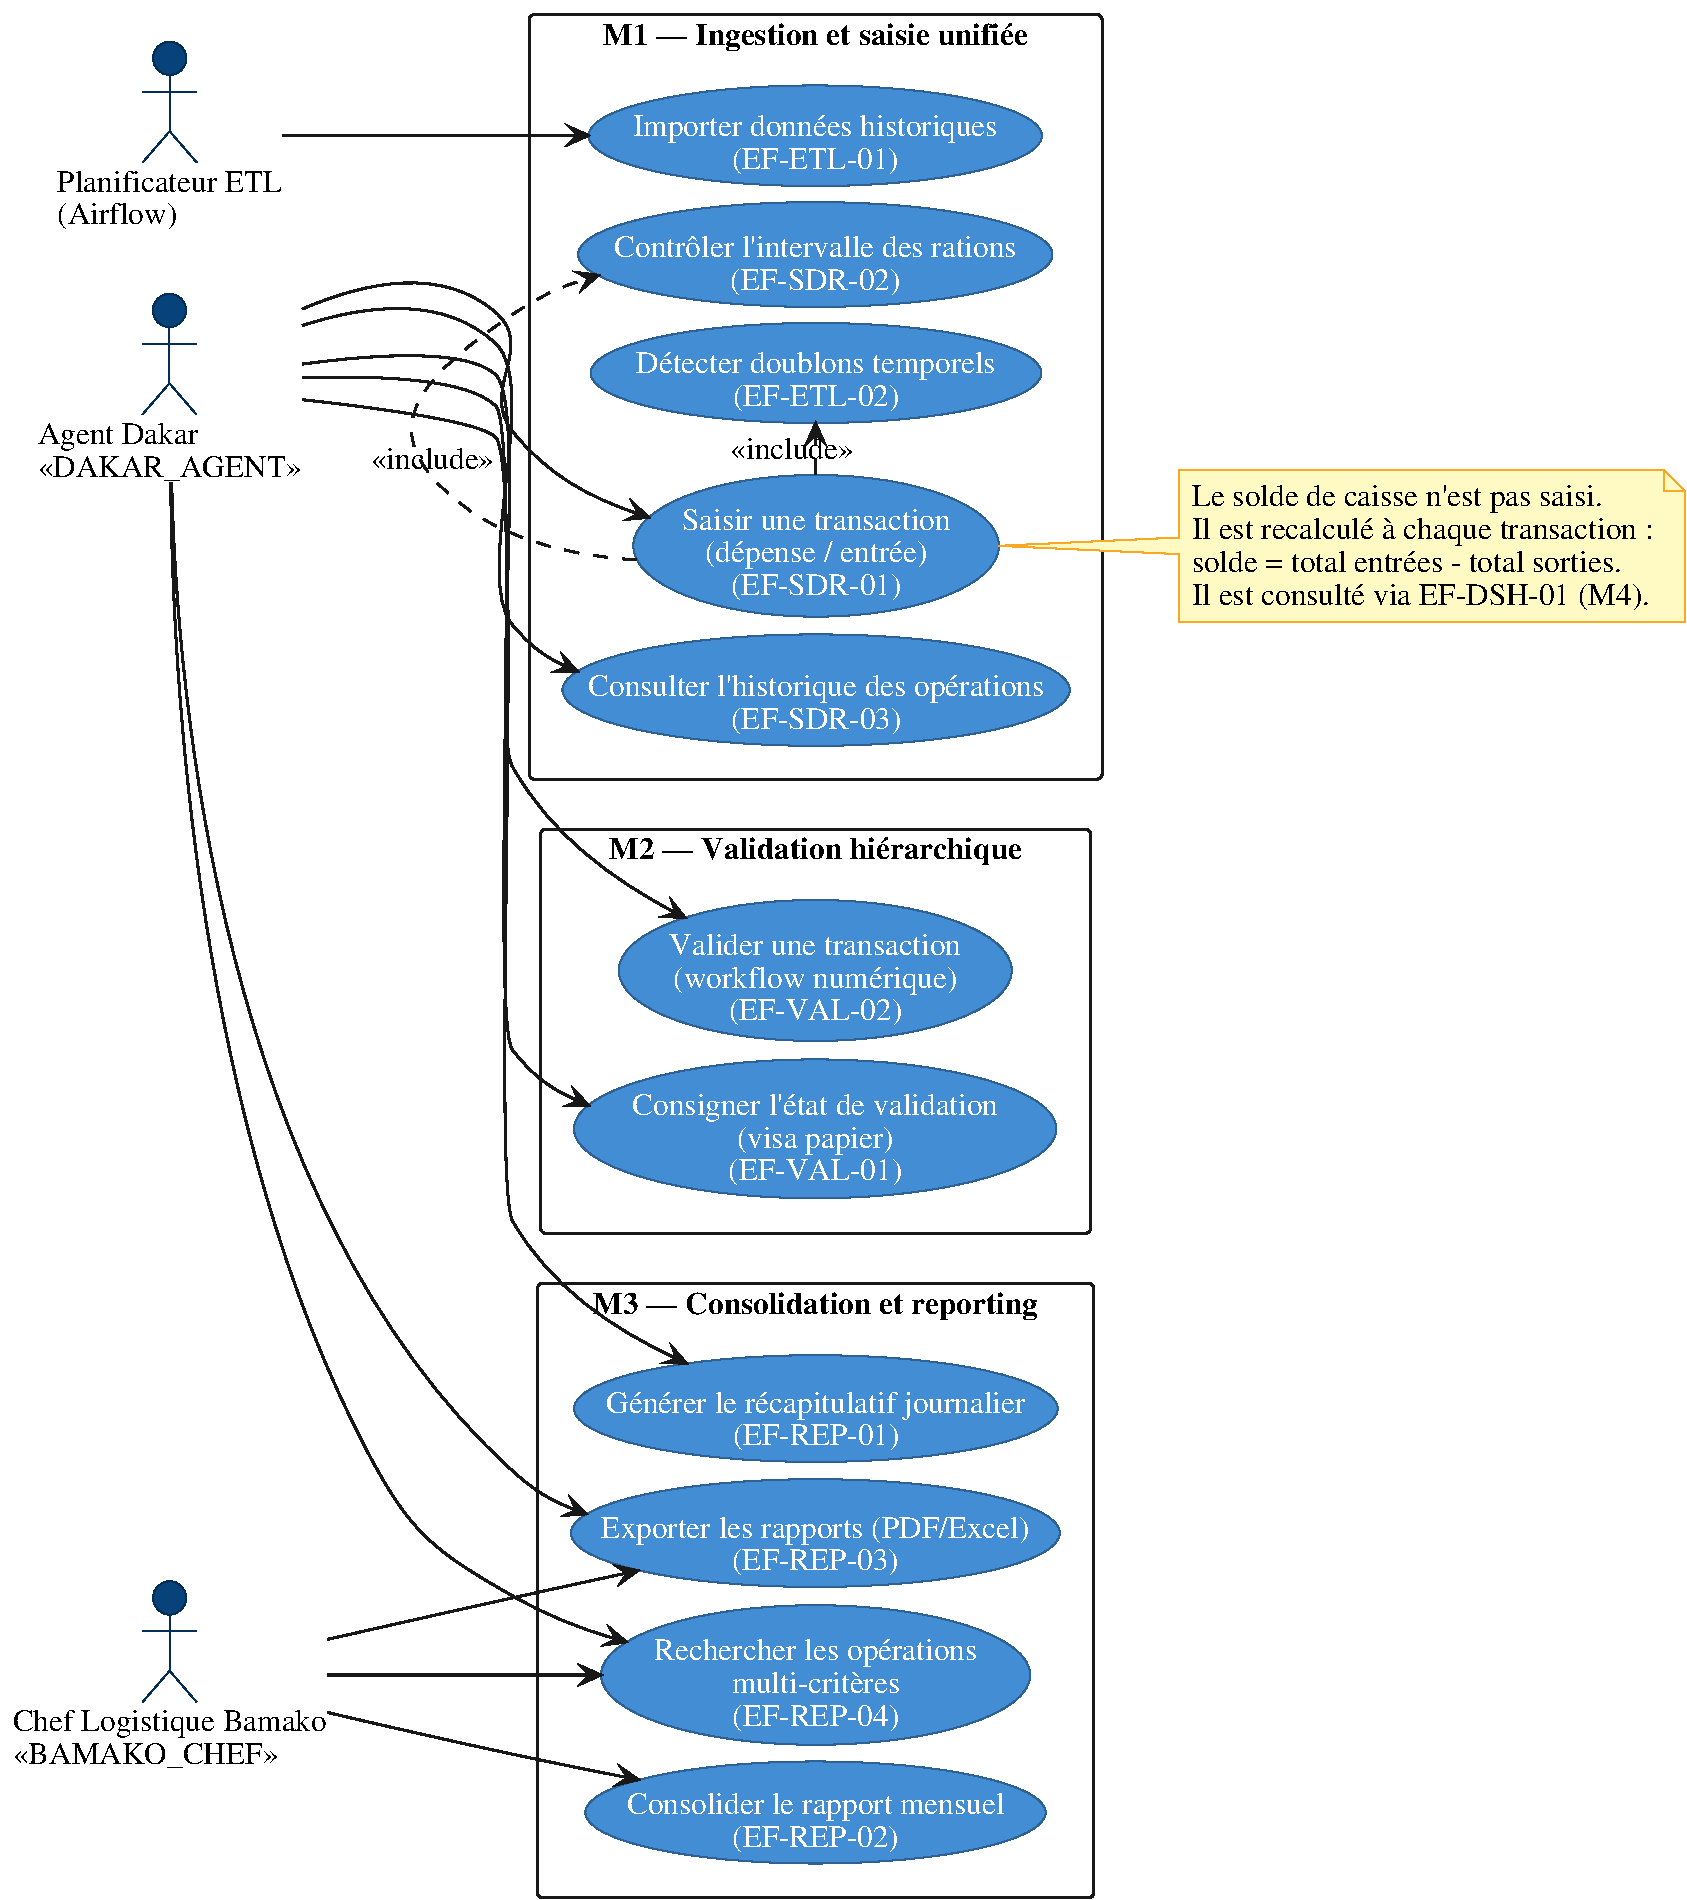
\includegraphics[width=\textwidth,height=0.88\textheight,keepaspectratio]{figures/fig_cas_utilisation_m1_m3.pdf}
    \caption{Diagramme de cas d'utilisation, modules M1 à M3 (Ingestion, Validation, Reporting), plateforme SOYAFF}
    \label{fig:cas_utilisation_1}
    \source{Schéma de l'auteur}
\end{figure}

\begin{figure}[H]
    \centering
    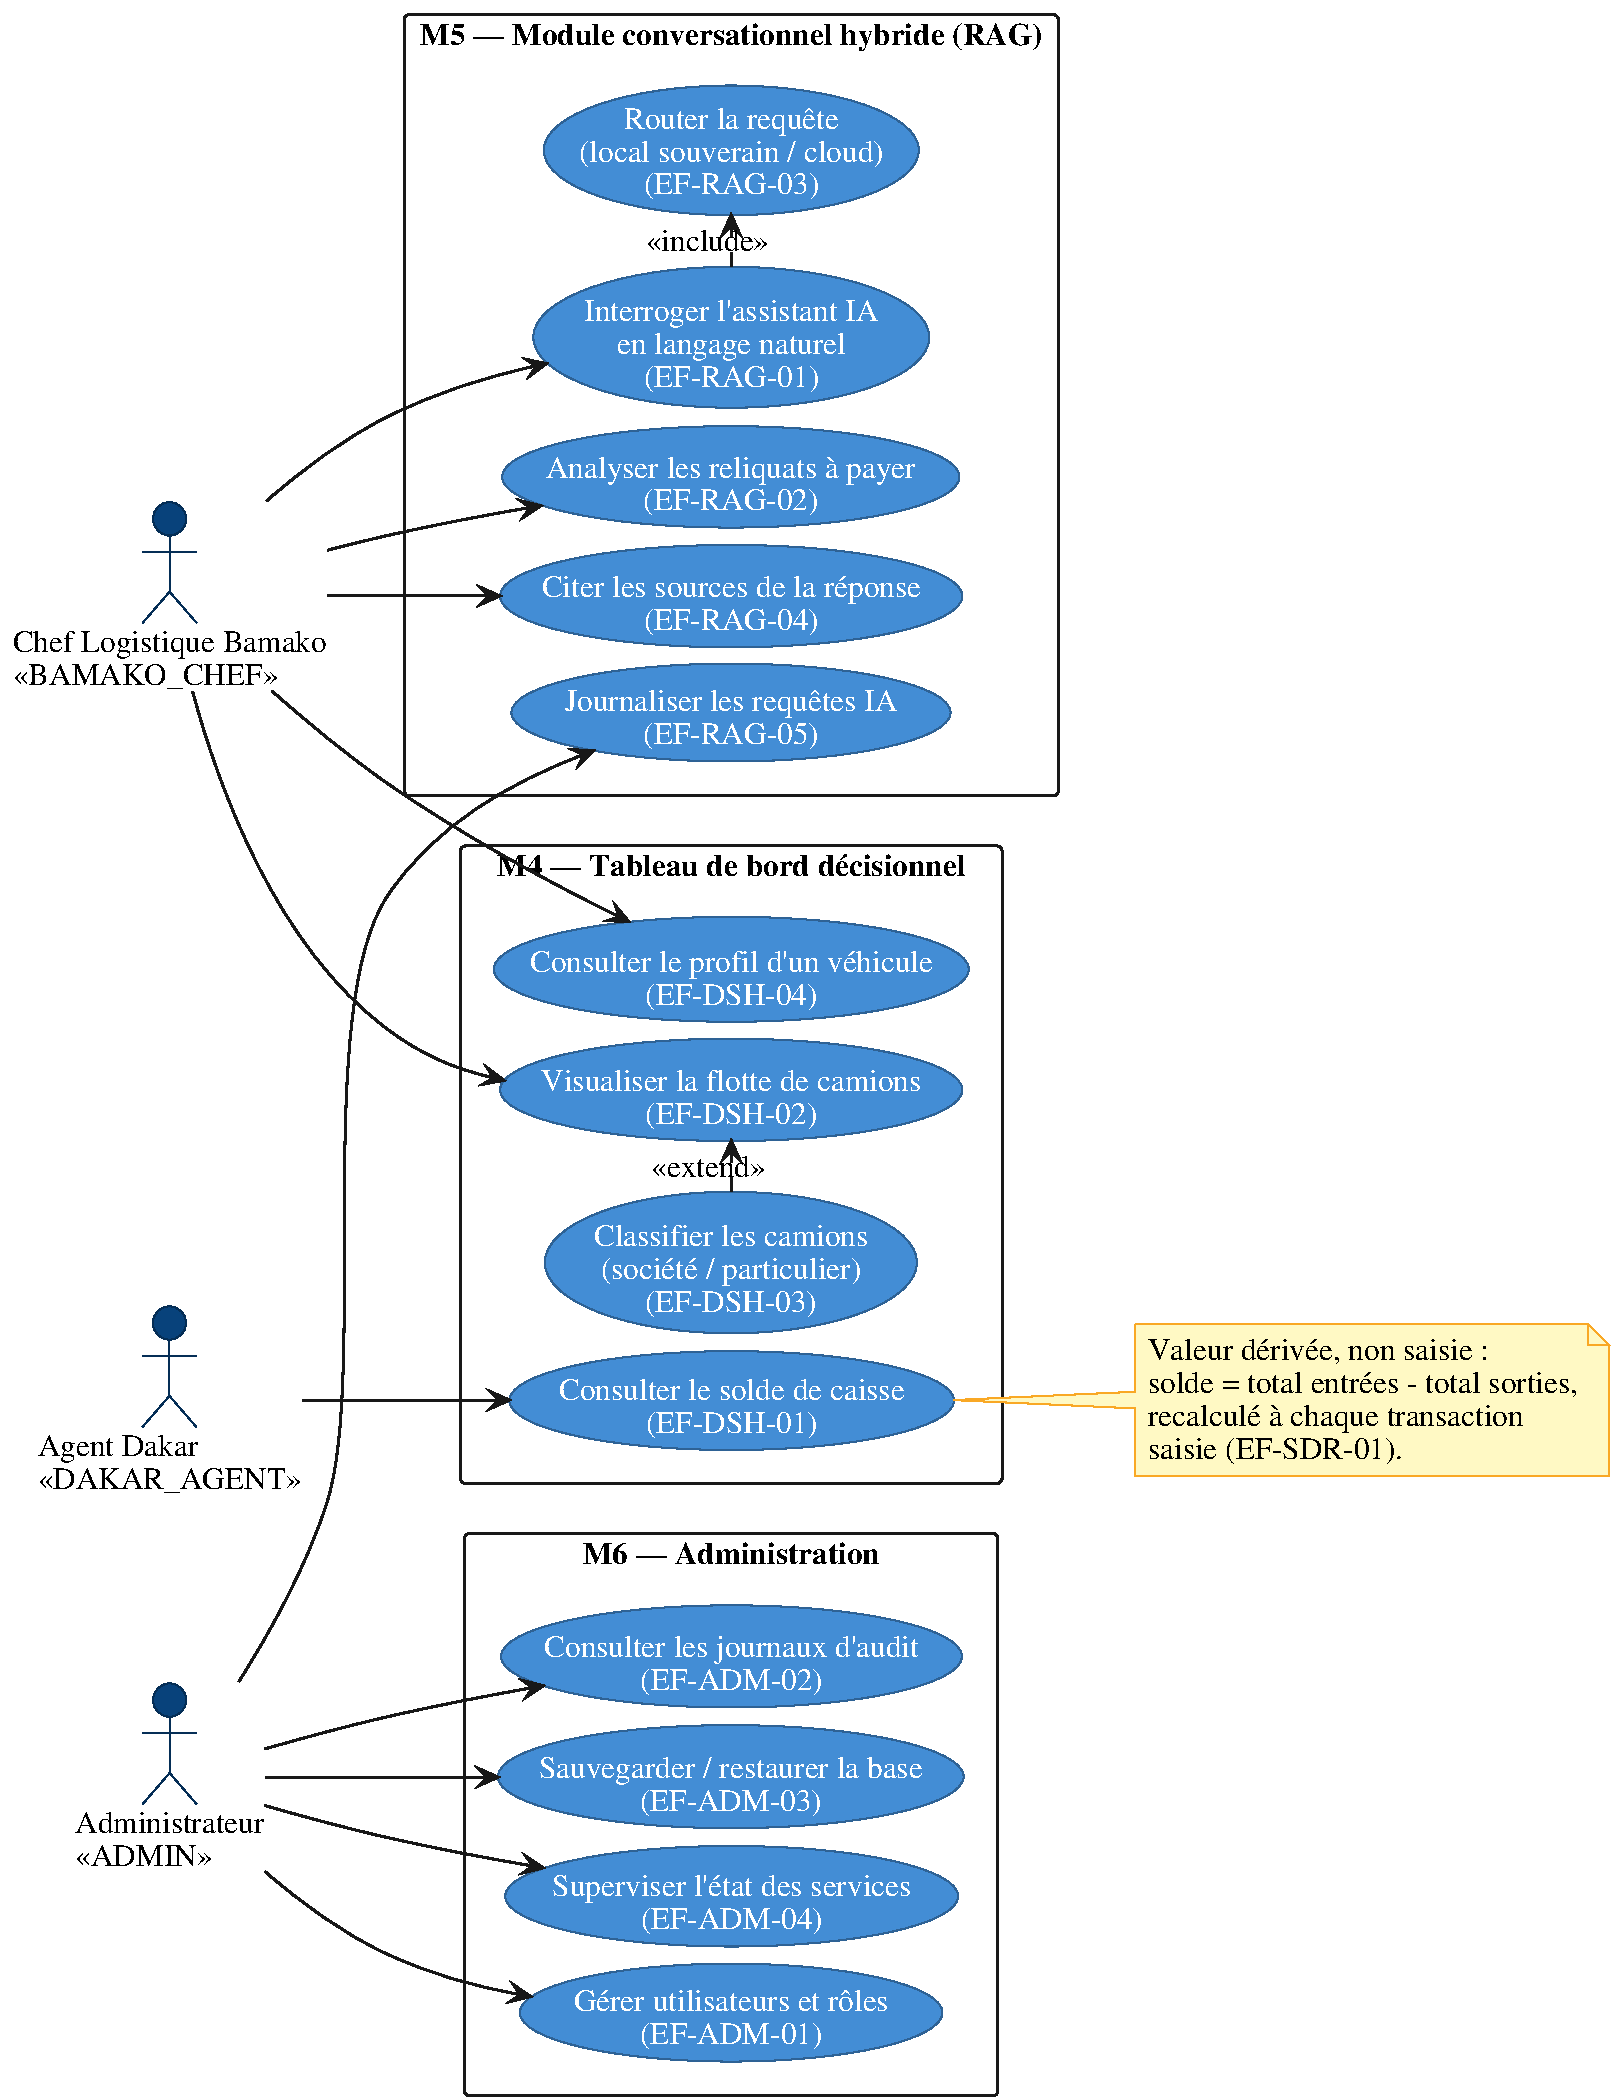
\includegraphics[width=\textwidth,height=0.88\textheight,keepaspectratio]{figures/fig_cas_utilisation_m4_m6.pdf}
    \caption{Diagramme de cas d'utilisation, modules M4 à M6 (Tableau de bord, RAG, Administration), plateforme SOYAFF}
    \label{fig:cas_utilisation_2}
    \source{Schéma de l'auteur}
\end{figure}

\subsection{Modèle de classes du domaine}
\label{sec:classes_domaine}
Le diagramme de classes du domaine métier (Figure~\ref{fig:classes_domaine}) modélise les concepts manipulés par la plateforme, à un niveau d'abstraction conceptuel et non celui du schéma physique de base de données présenté à la section~\ref{chap:architecture}. Les noms de classes et d'attributs sont volontairement alignés sur les tables et colonnes réelles de la base PostgreSQL, afin d'assurer la cohérence entre l'analyse et la réalisation. La classe \texttt{Validation} y figure avec le stéréotype \guillemotleft~conceptuel~\guillemotright~: elle matérialise les exigences \texttt{EF-VAL-01/02} sans préjuger d'une persistance déjà implémentée, cet aspect étant traité au chapitre~\ref{chap:realisation}.

Le modèle s'articule autour de la classe centrale \texttt{Transaction}, qui matérialise tout mouvement financier ou opérationnel. Une \texttt{Transaction} \emph{concerne} un \texttt{Camion} (multiplicité 1 côté camion, chaque camion pouvant porter un nombre indéterminé de transactions), lui-même \emph{conduit} par un \texttt{Chauffeur} : cette chaîne permet de reconstituer le coût réel par véhicule et par chauffeur, indicateur central absent du système actuel (cf. §\ref{sec:recueil}). La classe \texttt{BonLivraison} agrège les transactions relatives à un même chargement et est reliée aux \texttt{Produit} transportés par une association plusieurs-à-plusieurs, un bon regroupant plusieurs références et une référence figurant sur plusieurs bons. Cette association porte une donnée qui n'appartient ni au bon ni au produit, la quantité livrée : elle est donc modélisée par la classe d'association \texttt{BonLivraisonProduit}, rattachée au lien entre les deux classes. L'attribut \texttt{/solde\_progressif} de \texttt{Transaction} est noté comme attribut dérivé : il n'est jamais saisi, mais calculé à partir des entrées et des sorties. Enfin, la classe \texttt{Validation}, ici purement conceptuelle, s'attache à la \texttt{Transaction} qu'elle qualifie sans en présumer la persistance physique. Les classes \texttt{Utilisateur}, \texttt{RequeteIA} et \texttt{AuditLog} constituent le socle transverse de sécurité et de traçabilité (RBAC, journalisation IA et piste d'audit) exigé par les \texttt{ENF-SEC} et \texttt{EF-RAG-05}. L'ensemble \texttt{CategorieOperation} est modélisé comme une énumération (et non une entité), reflétant son statut de colonne typée dans le schéma relationnel.

\begin{landscape}
\begin{figure}[p]
    \centering
    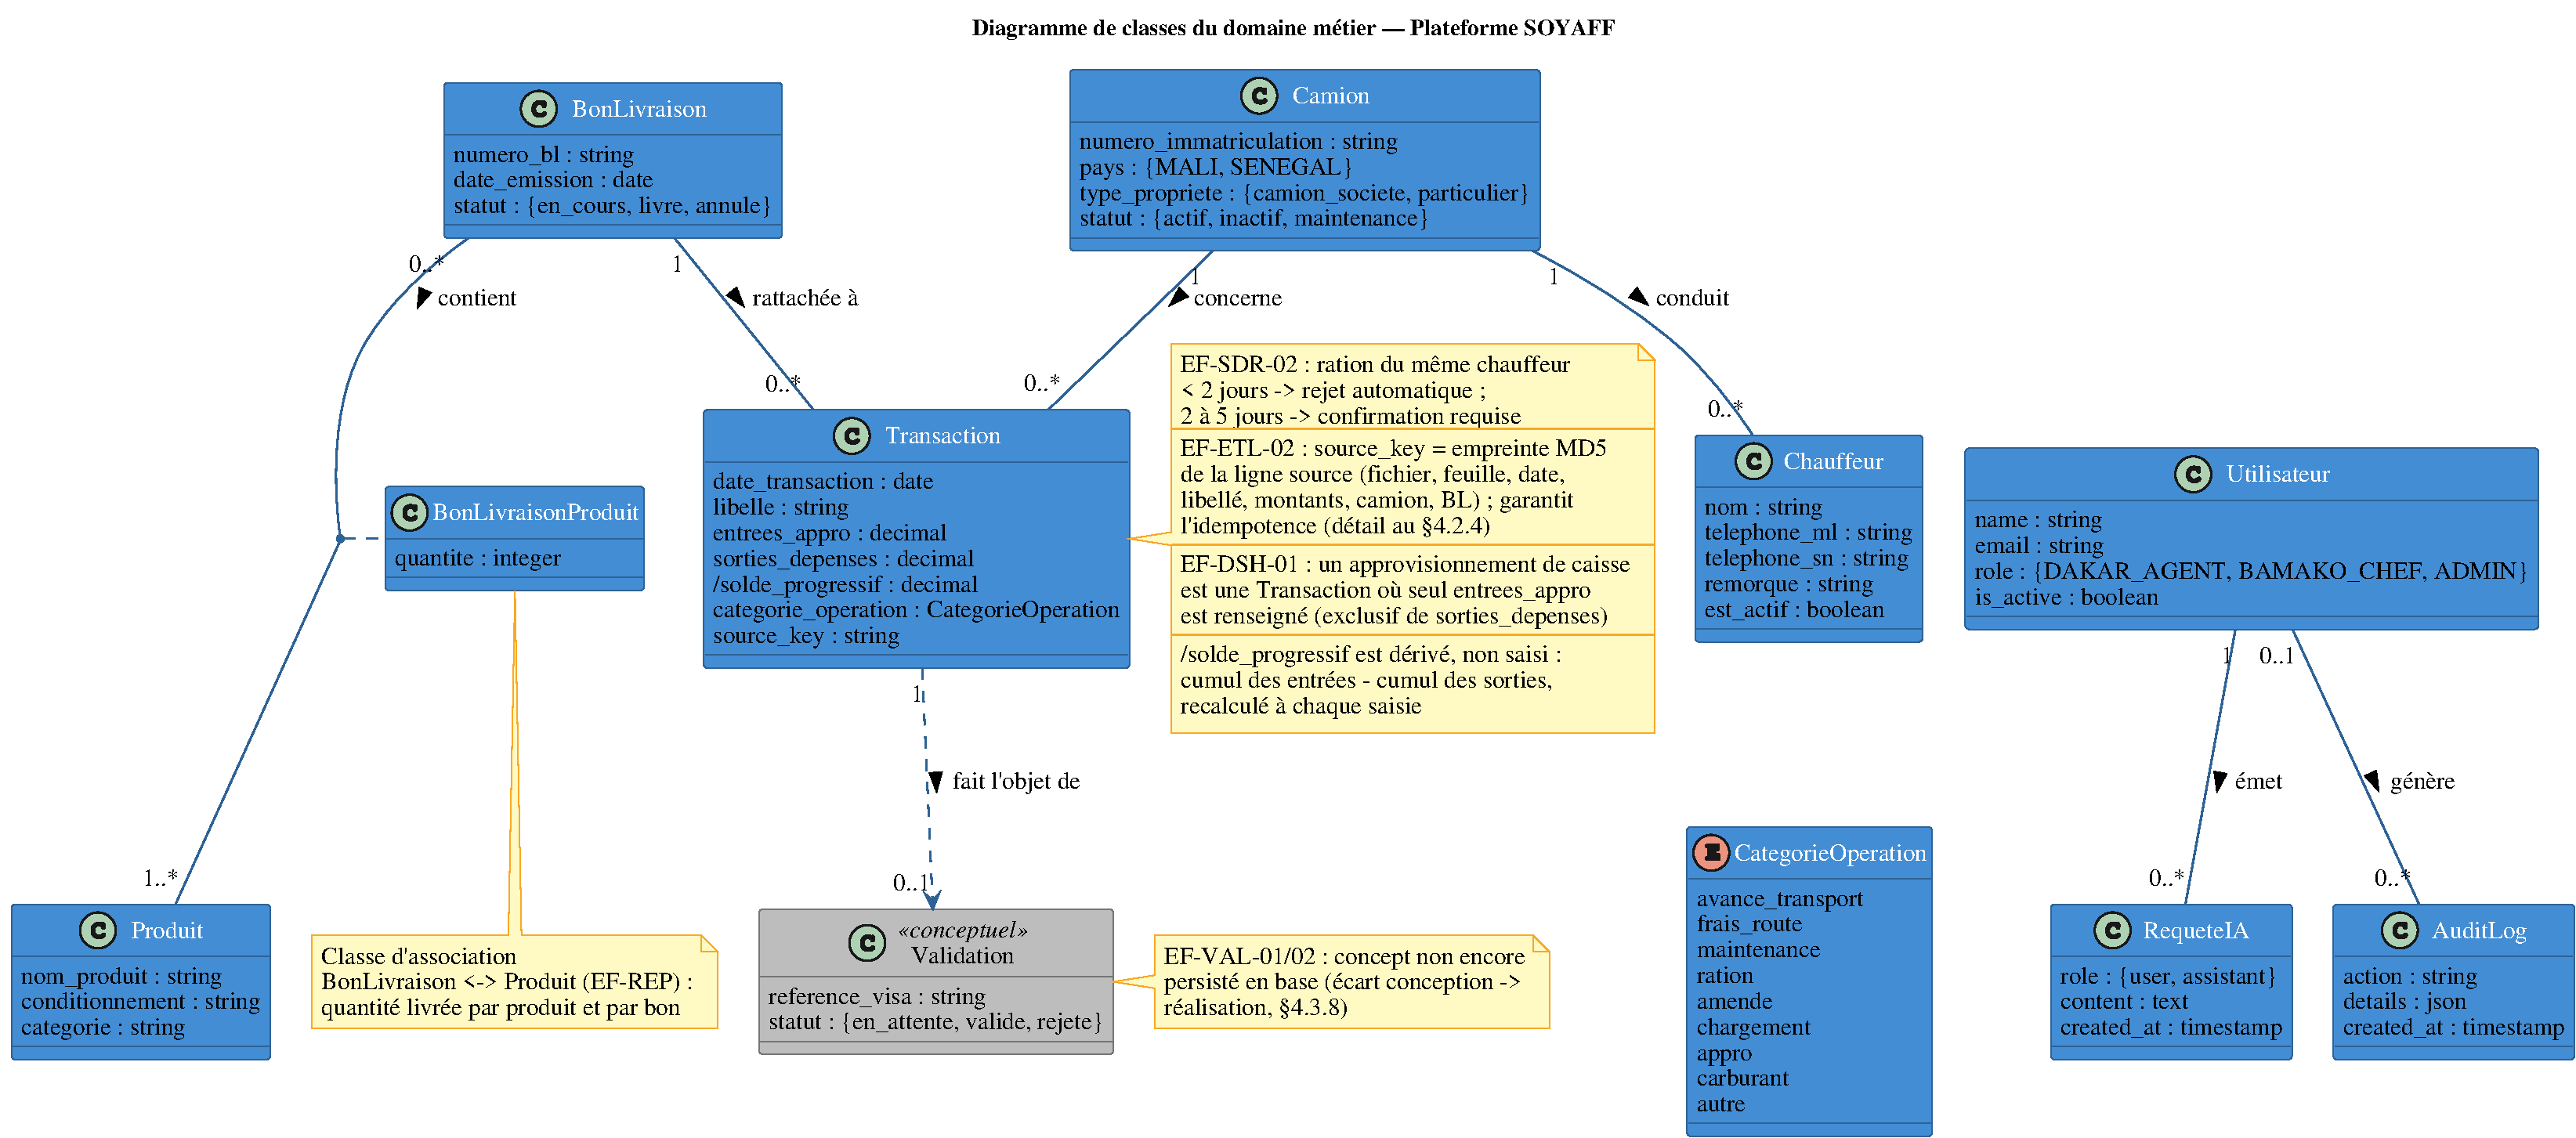
\includegraphics[width=\linewidth,height=0.86\textheight,keepaspectratio]{figures/fig_classes_domaine.pdf}
    \caption{Diagramme de classes du domaine métier, plateforme SOYAFF}
    \label{fig:classes_domaine}
    \source{Schéma de l'auteur}
\end{figure}
\end{landscape}

\subsection{Comportements dynamiques}
\label{sec:sequences}
Les deux scénarios suivants ont été retenus pour leur caractère structurant : le premier opérationnalise les garde-fous métier de la saisie (§\ref{sec:recueil}), le second matérialise la définition d'architecture \guillemotleft~hybride~\guillemotright~qui porte l'hypothèse H2.

\subsubsection{Séquence de saisie d'une dépense avec contrôles}
\label{subsec:seq_saisie}
La Figure~\ref{fig:seq_saisie} détaille le scénario de saisie d'une dépense, avec ses deux garde-fous : la détection de doublons temporels (\texttt{EF-ETL-02}) et le contrôle de l'intervalle entre deux rations (\texttt{EF-SDR-02}), modélisés par des fragments combinés \texttt{alt}.

\begin{figure}[H]
    \centering
    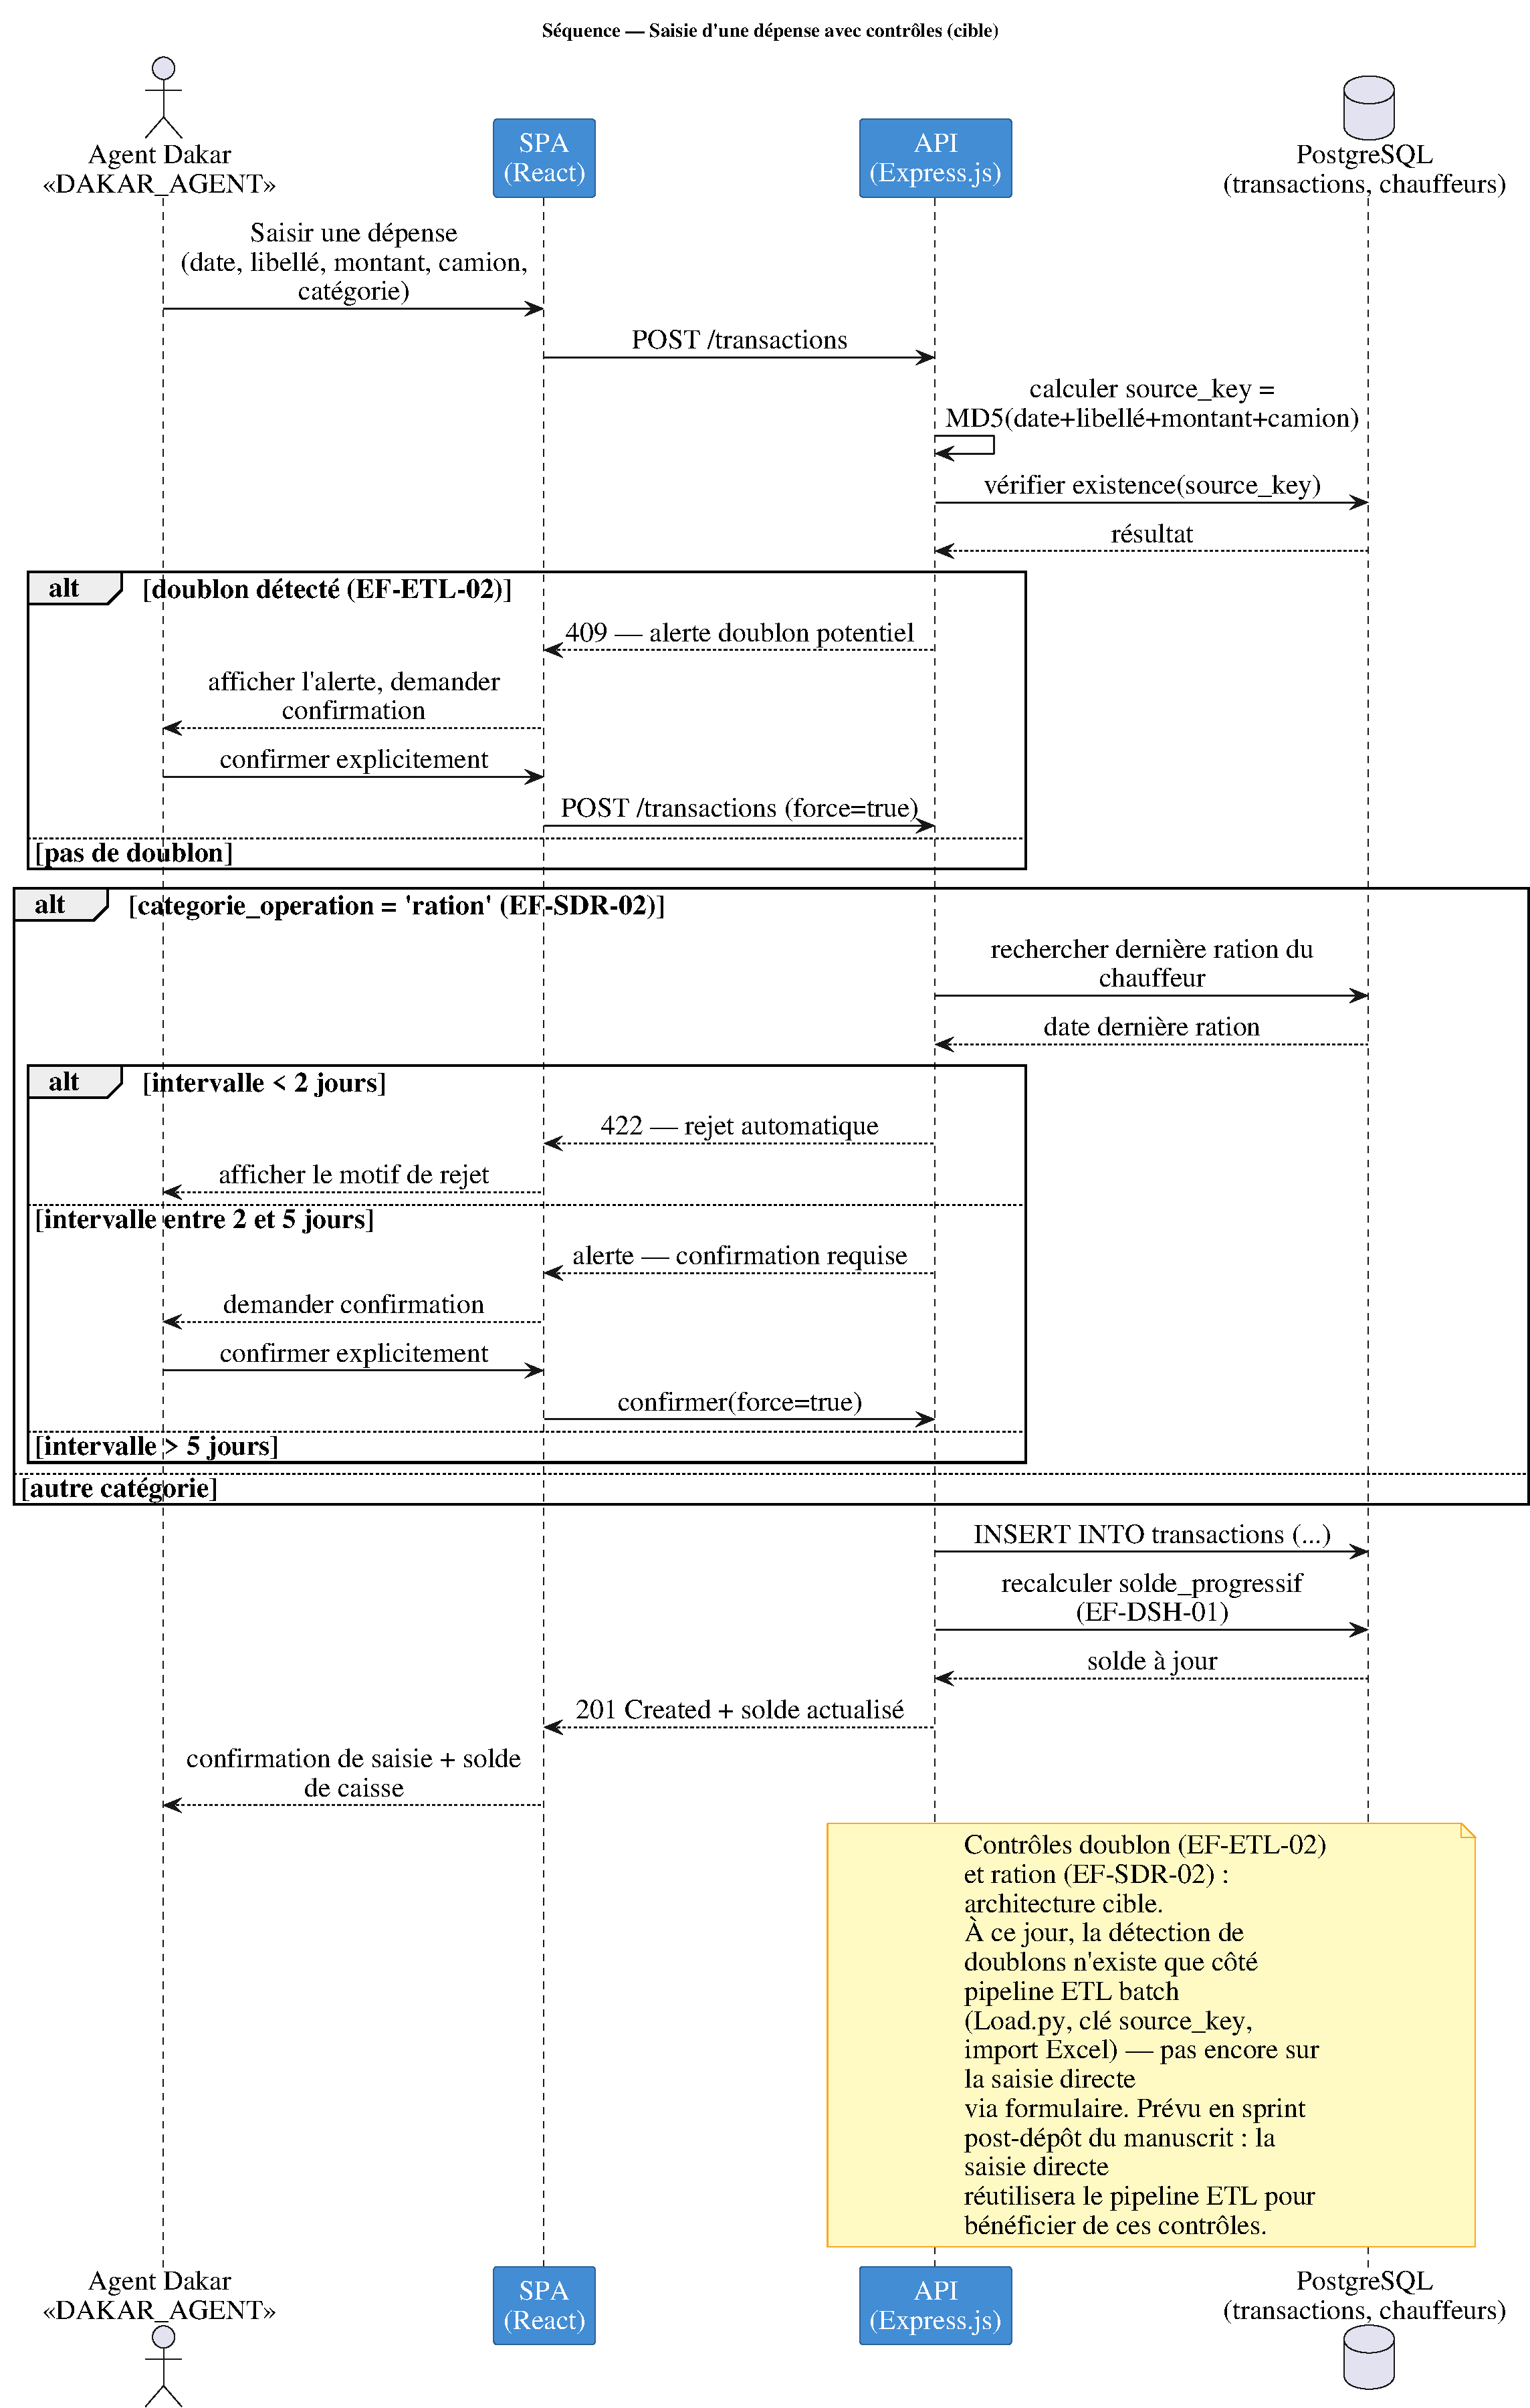
\includegraphics[width=\textwidth,height=0.88\textheight,keepaspectratio]{figures/fig_seq_saisie_controles.pdf}
    \caption{Séquence : saisie d'une dépense avec contrôles}
    \label{fig:seq_saisie}
    \source{Schéma de l'auteur}
\end{figure}

\subsubsection{Séquence de requête RAG avec routage hybride}
\label{subsec:seq_rag}
La Figure~\ref{fig:seq_rag} illustre le traitement d'une requête en langage naturel adressée à l'agent conversationnel, depuis sa soumission jusqu'à la restitution de la réponse. Le routage entre chemin local souverain et chemin cloud (\texttt{EF-RAG-03}) y est représenté par un fragment \texttt{alt} conditionné par l'analyse de sensibilité réalisée par l'orchestrateur n8n.

\begin{landscape}
\begin{figure}[p]
    \centering
    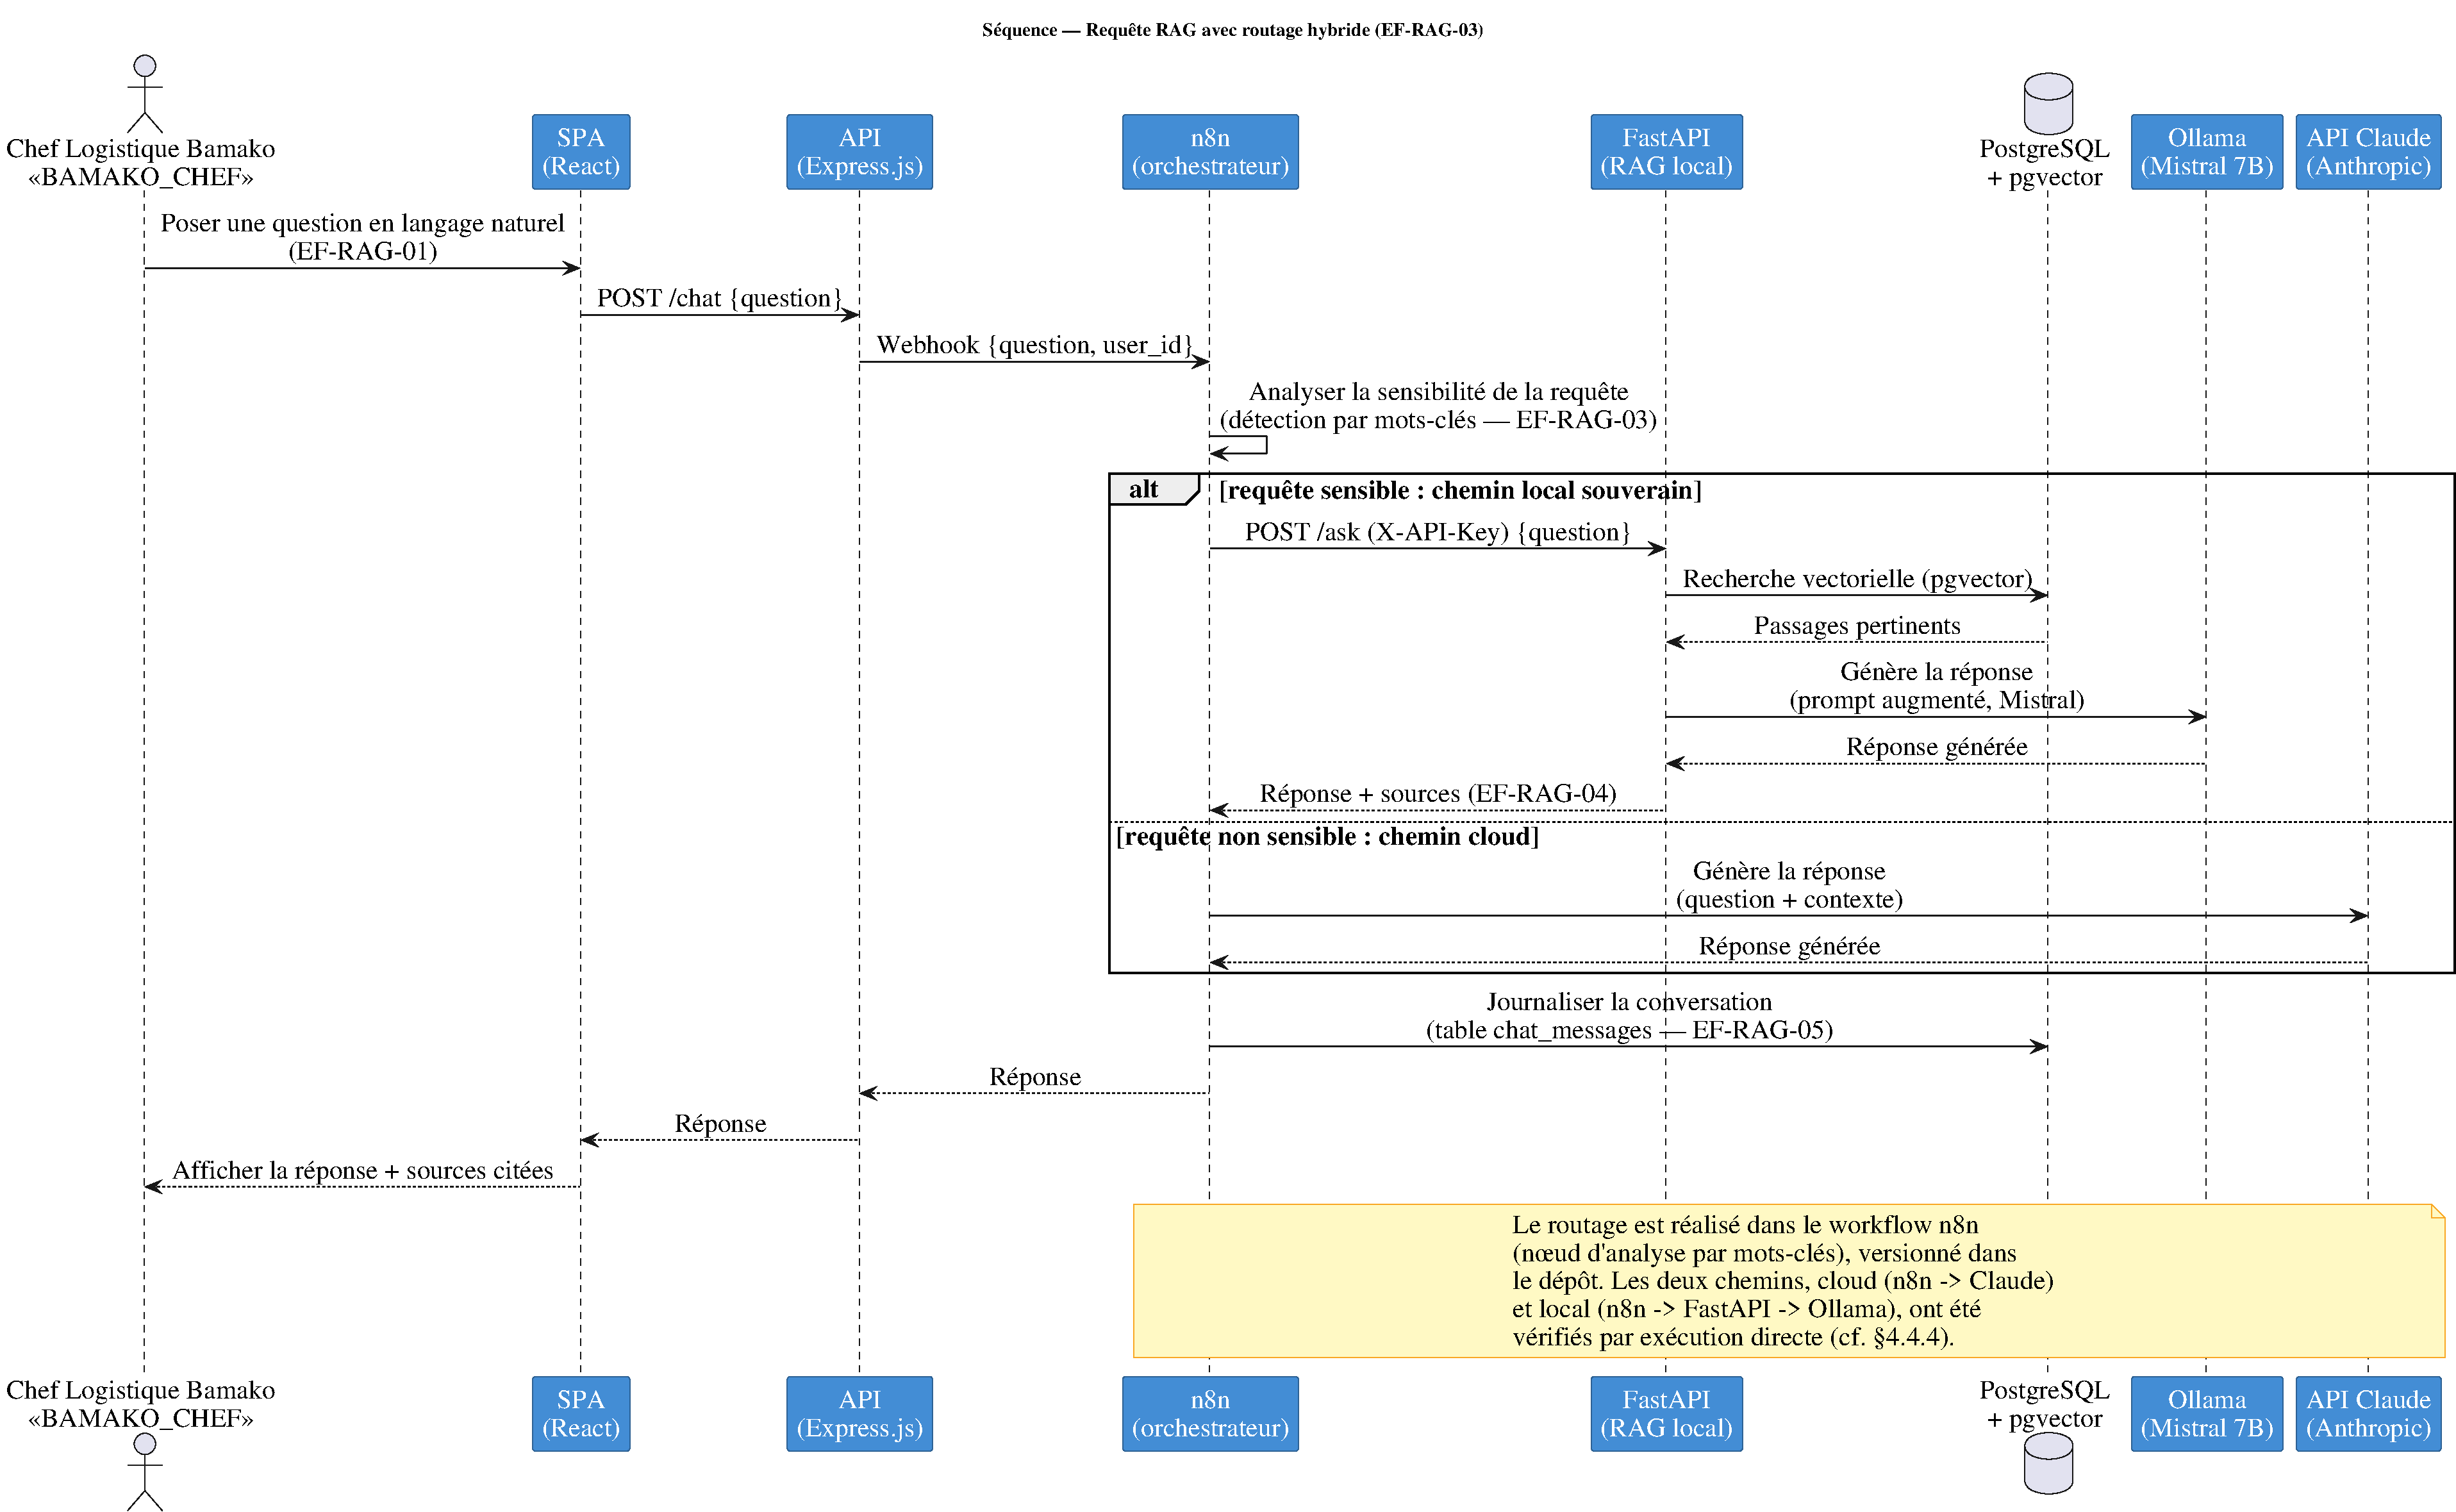
\includegraphics[width=\linewidth,height=0.86\textheight,keepaspectratio]{figures/fig_seq_rag_hybride.pdf}
    \caption{Séquence : requête RAG avec routage hybride}
    \label{fig:seq_rag}
    \source{Schéma de l'auteur}
\end{figure}
\end{landscape}

\subsection{Workflow de validation}
\label{sec:activite_validation}
Les deux séquences précédentes décrivent des interactions synchrones, centrées sur une requête unique. Le processus de validation, lui, est un flux de travail asynchrone avec plusieurs acteurs et des points de décision : le diagramme d'activité est le formalisme adapté.

Les Figures~\ref{fig:activite_validation_actuelle} et~\ref{fig:activite_validation_cible} présentent, sous forme de diagrammes d'activité à couloirs, le circuit de validation observé sur le terrain et le circuit dématérialisé cible. Le premier correspond à l'exigence \textit{Must} \texttt{EF-VAL-01} ; le second, à l'exigence \textit{Should} \texttt{EF-VAL-02}, dont la priorisation reflète le maintien du circuit papier comme référence juridiquement opposable durant la phase de transition (§\ref{sec:synthese_tracabilite}).

\begin{figure}[H]
    \centering
    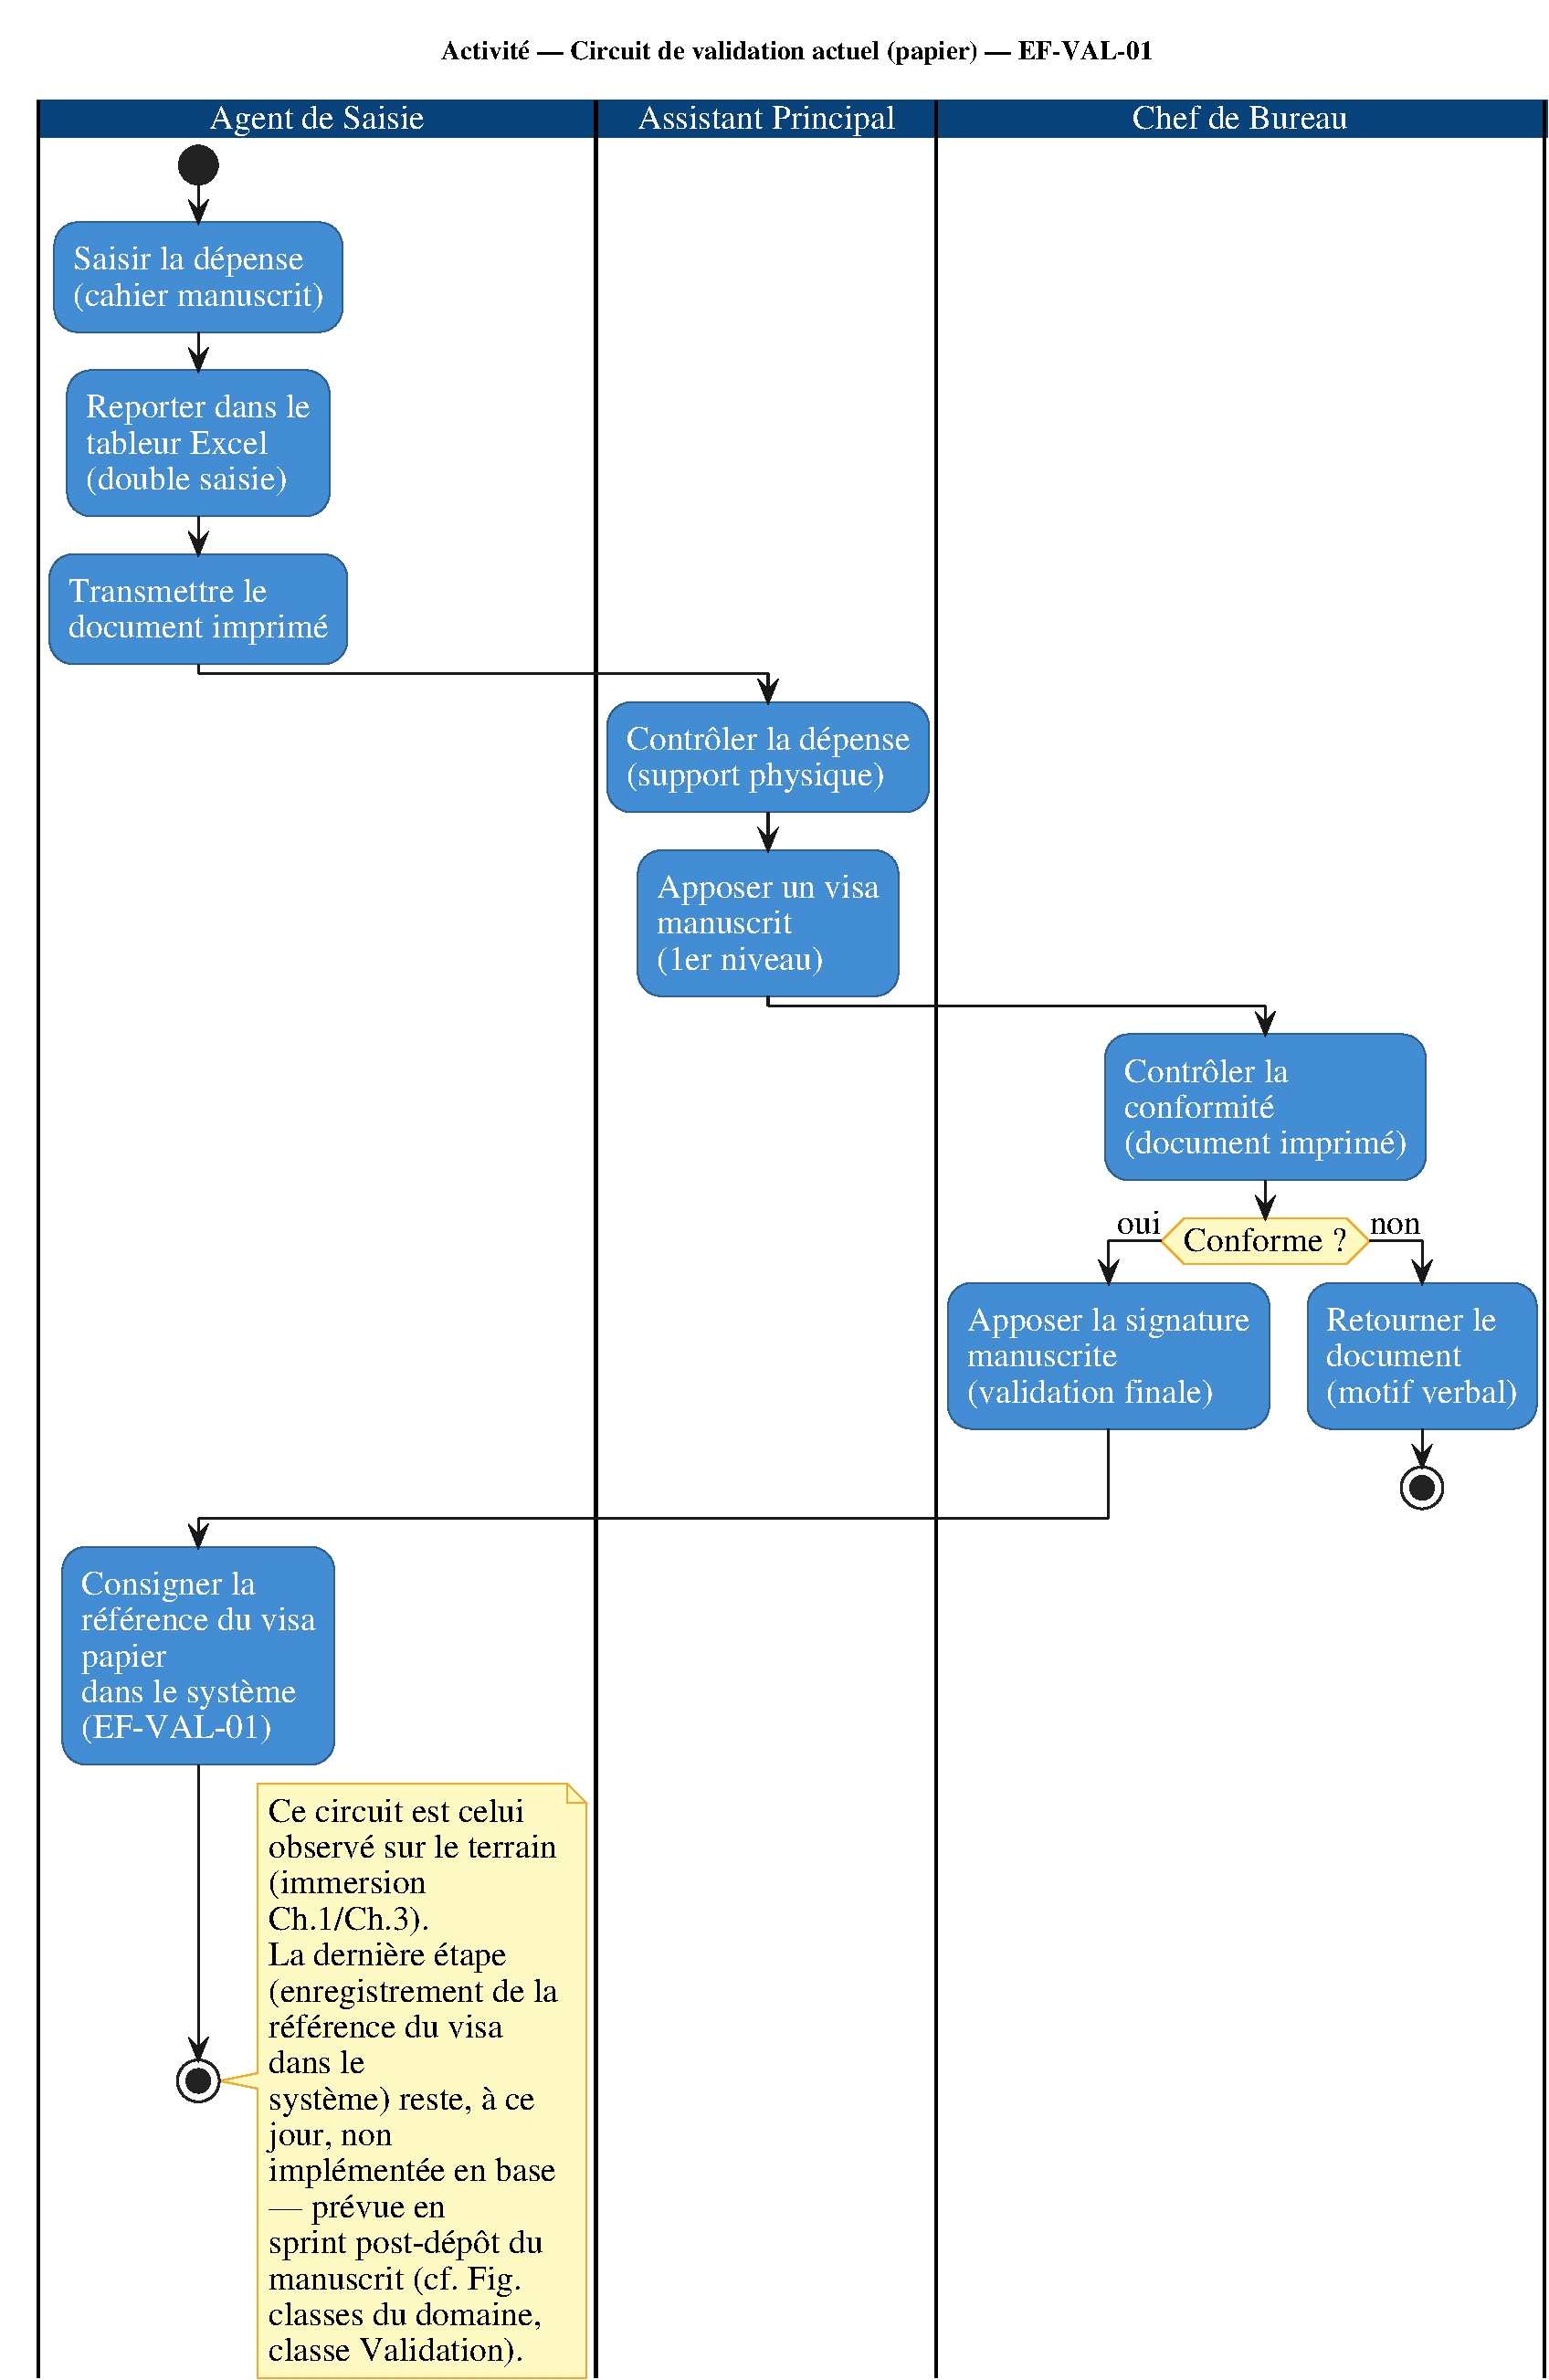
\includegraphics[width=\textwidth,height=0.88\textheight,keepaspectratio]{figures/fig_activite_validation_actuelle.pdf}
    \caption{Activité : circuit de validation actuel (papier)}
    \label{fig:activite_validation_actuelle}
    \source{Schéma de l'auteur}
\end{figure}

\begin{figure}[H]
    \centering
    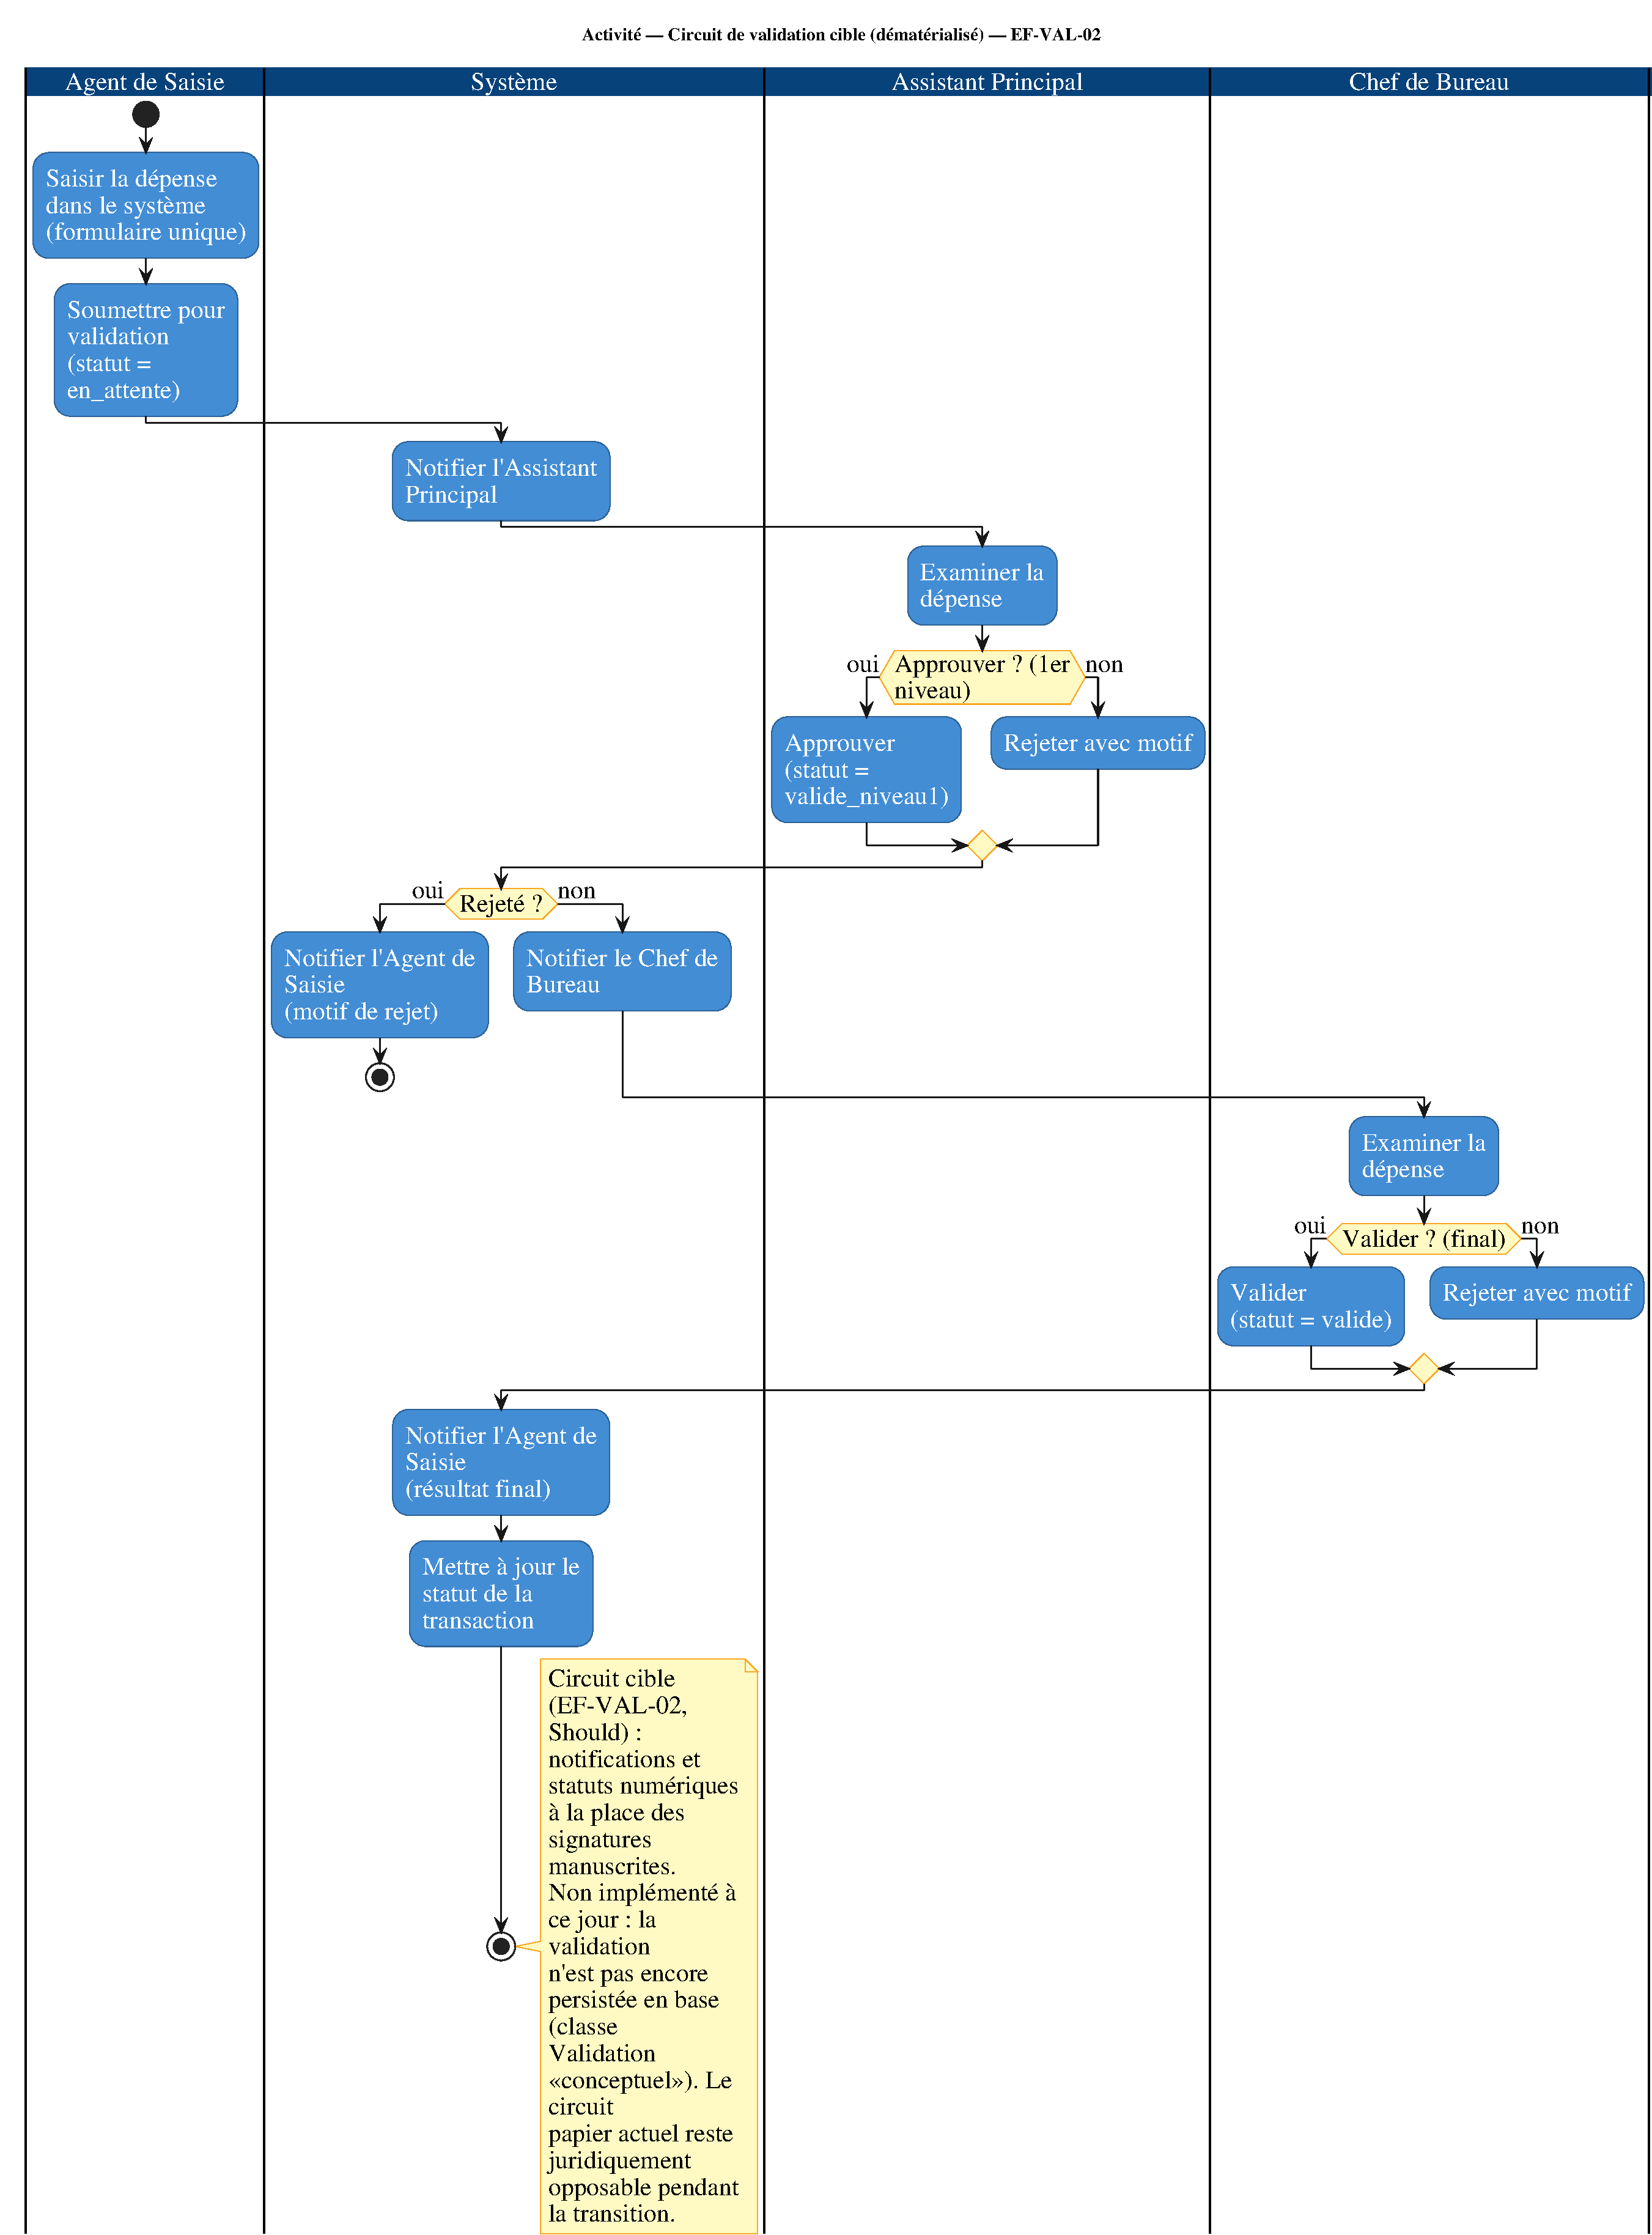
\includegraphics[width=\textwidth,height=0.88\textheight,keepaspectratio]{figures/fig_activite_validation_cible.pdf}
    \caption{Activité : circuit de validation cible (dématérialisé)}
    \label{fig:activite_validation_cible}
    \source{Schéma de l'auteur}
\end{figure}


\section{Architecture de la solution (C4 et ADR)}
\label{chap:architecture}

Cette section présente l'architecture logicielle et d'infrastructure retenue pour la plateforme SOYAFF, selon les trois premiers niveaux du modèle C4 (contexte, conteneurs, composants), complétés par une vue de déploiement de l'infrastructure de production.

\subsection{Vue de contexte}
\label{sec:c4_contexte}
La Figure~\ref{fig:c4_contexte} situe la plateforme SOYAFF parmi les systèmes avec lesquels elle interagit : les trois rôles utilisateurs, l'API Claude d'Anthropic pour le traitement cloud des requêtes non sensibles (\texttt{EF-RAG-03}), les fichiers Excel legacy servant de source à l'import historique (\texttt{EF-ETL-01}), et l'application \texttt{kiri.app} déjà en usage, dont le périmètre disjoint est explicitement représenté (§\ref{sec:recueil}).

\begin{figure}[H]
    \centering
    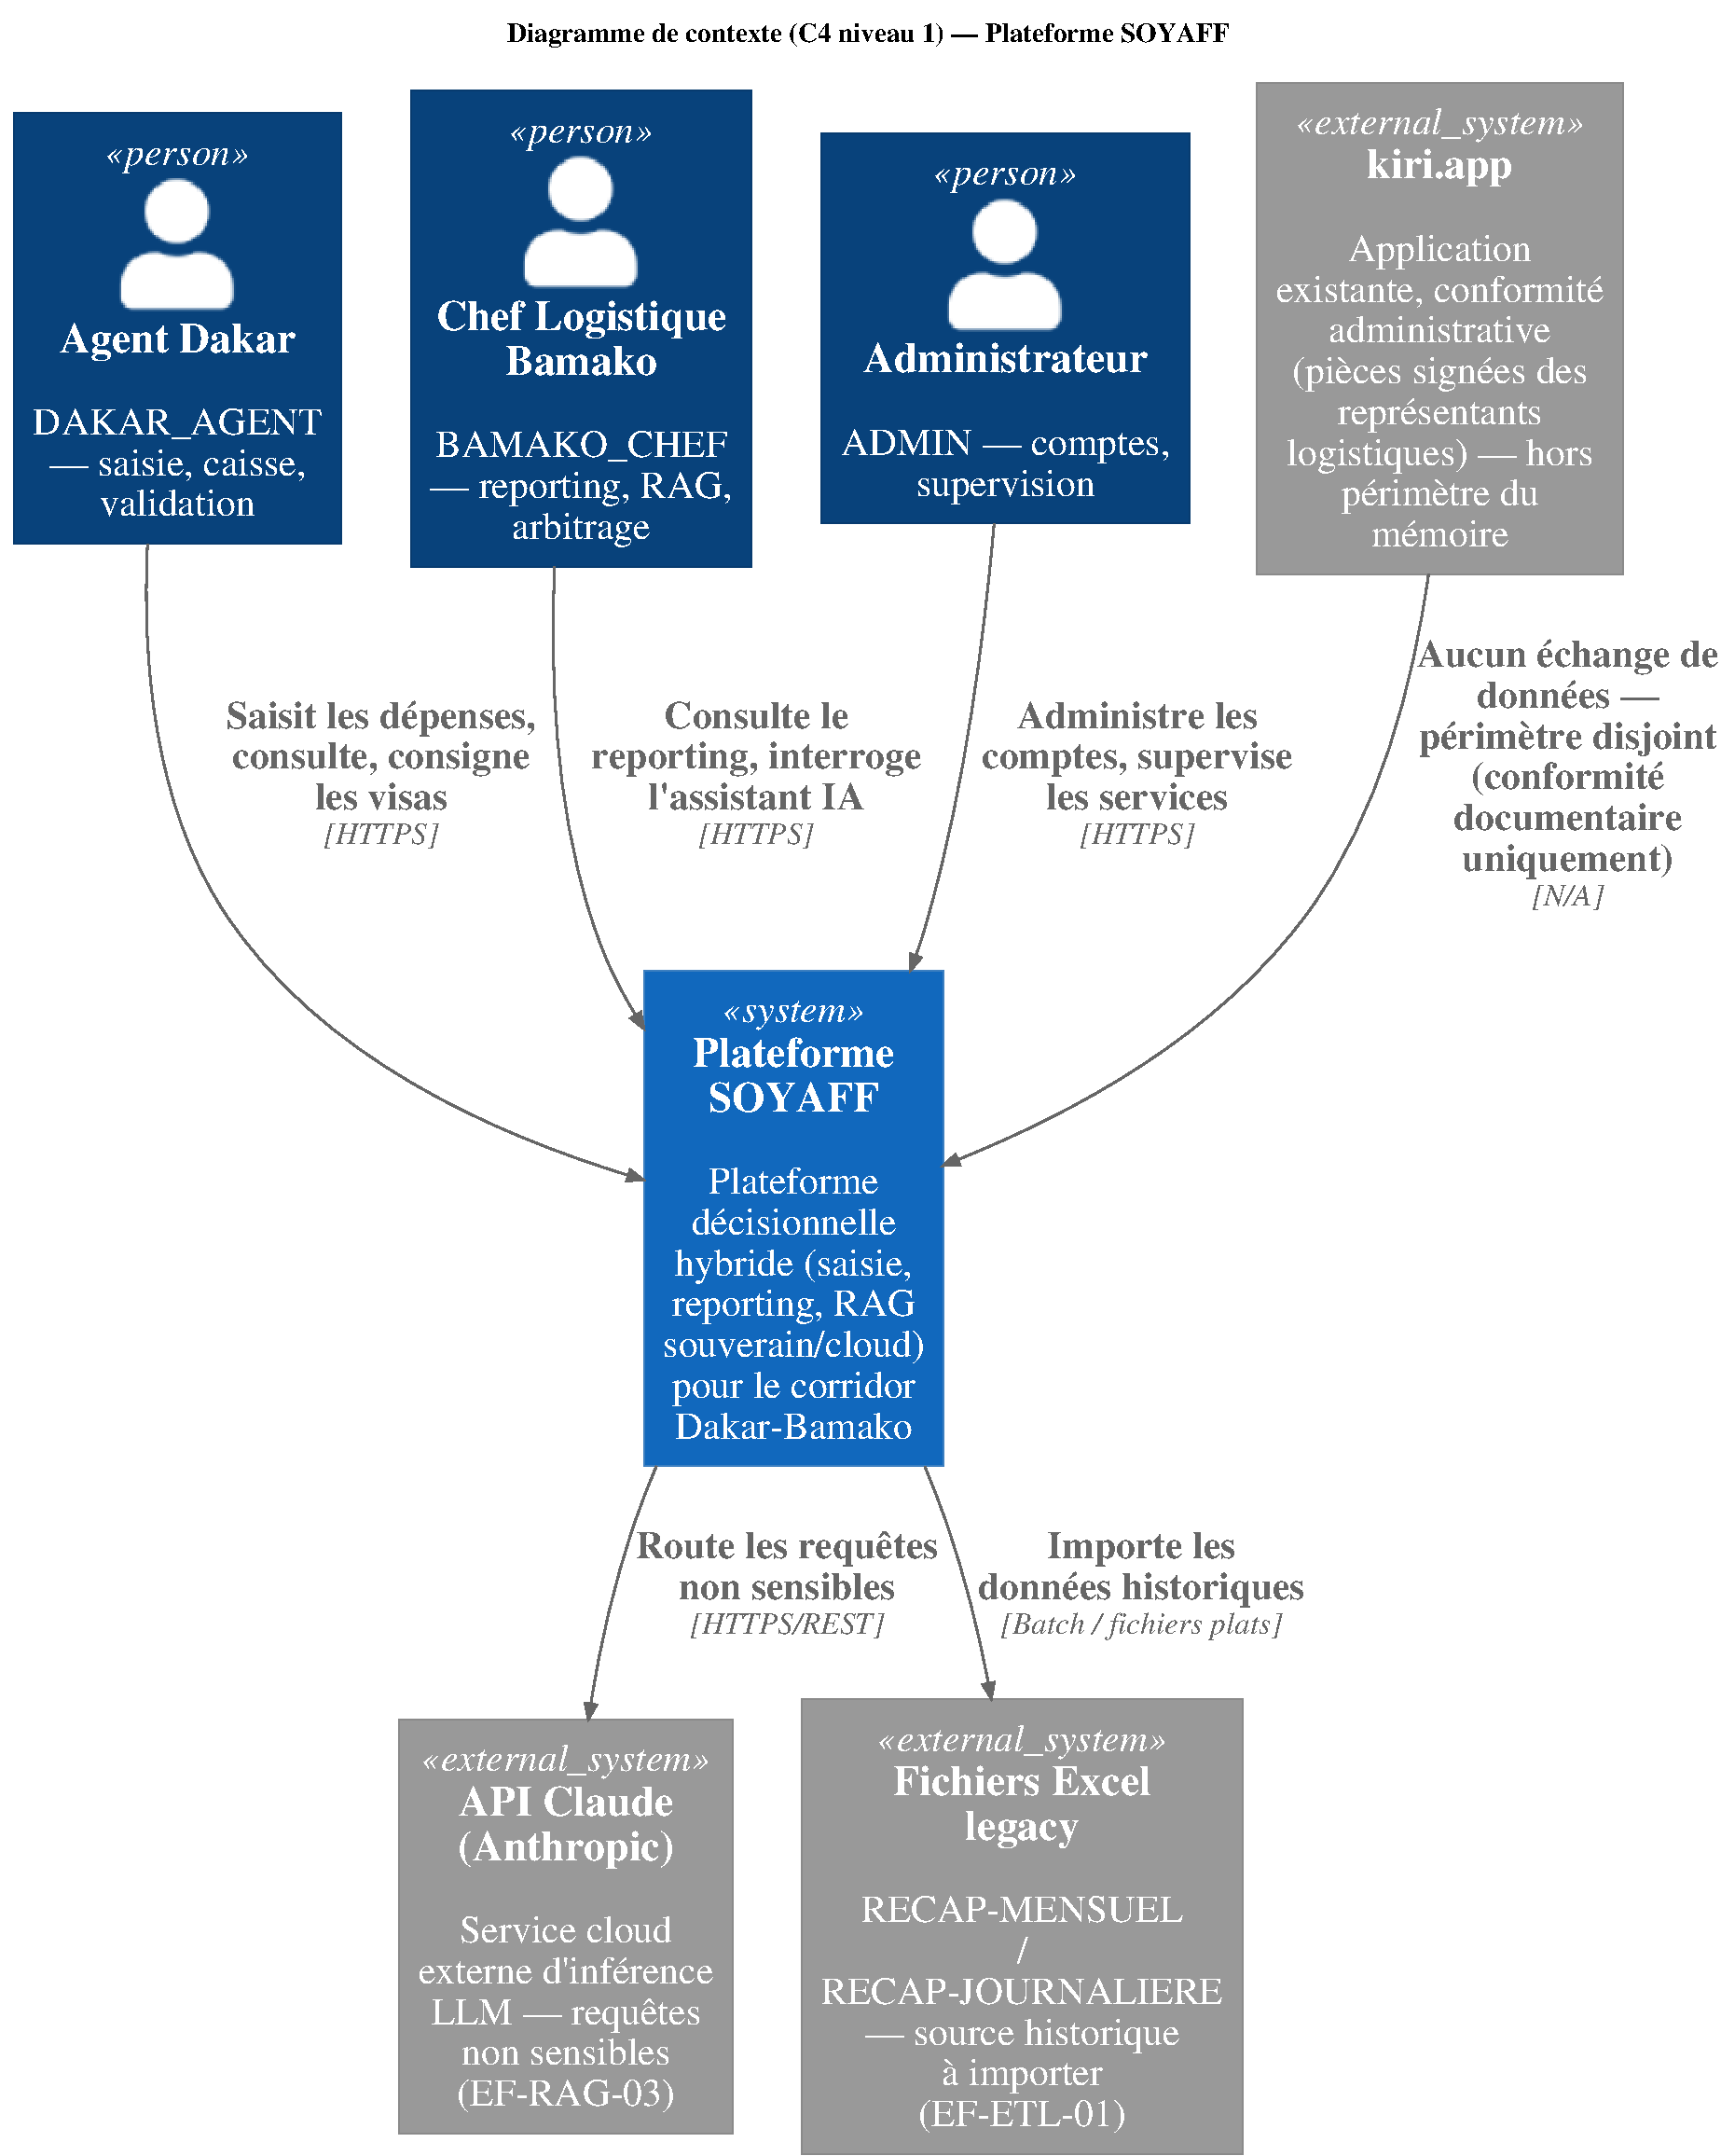
\includegraphics[width=\textwidth,height=0.88\textheight,keepaspectratio]{figures/fig_c4_contexte.pdf}
    \caption{Diagramme de contexte (C4 niveau 1), plateforme SOYAFF}
    \label{fig:c4_contexte}
    \source{Schéma de l'auteur}
\end{figure}

\subsection{Vue de conteneurs}
\label{sec:c4_conteneurs}
La Figure~\ref{fig:c4_conteneurs} détaille les conteneurs applicatifs déployés au sein du périmètre souverain de la plateforme. Le point d'entrée unique du module conversationnel est l'orchestrateur n8n, qui analyse la sensibilité de chaque requête et la route vers le service RAG local (FastAPI, Ollama/Mistral) ou vers l'API Claude cloud, conformément à \texttt{EF-RAG-03}. La conversation est journalisée en base (\texttt{EF-RAG-05}) indépendamment du chemin emprunté.

La frontière «\,périmètre souverain\,» tracée sur la figure n'est pas cosmétique : elle délimite l'ensemble des conteneurs au sein desquels les données métier ne quittent jamais l'infrastructure maîtrisée. Seul le chemin cloud (API Claude) la franchit, et uniquement pour des requêtes préalablement classées non sensibles par l'orchestrateur. Cette étanchéité conditionne la validité des exigences \texttt{ENF-SOUV-01} et \texttt{ENF-SOUV-02}.

\begin{figure}[H]
    \centering
    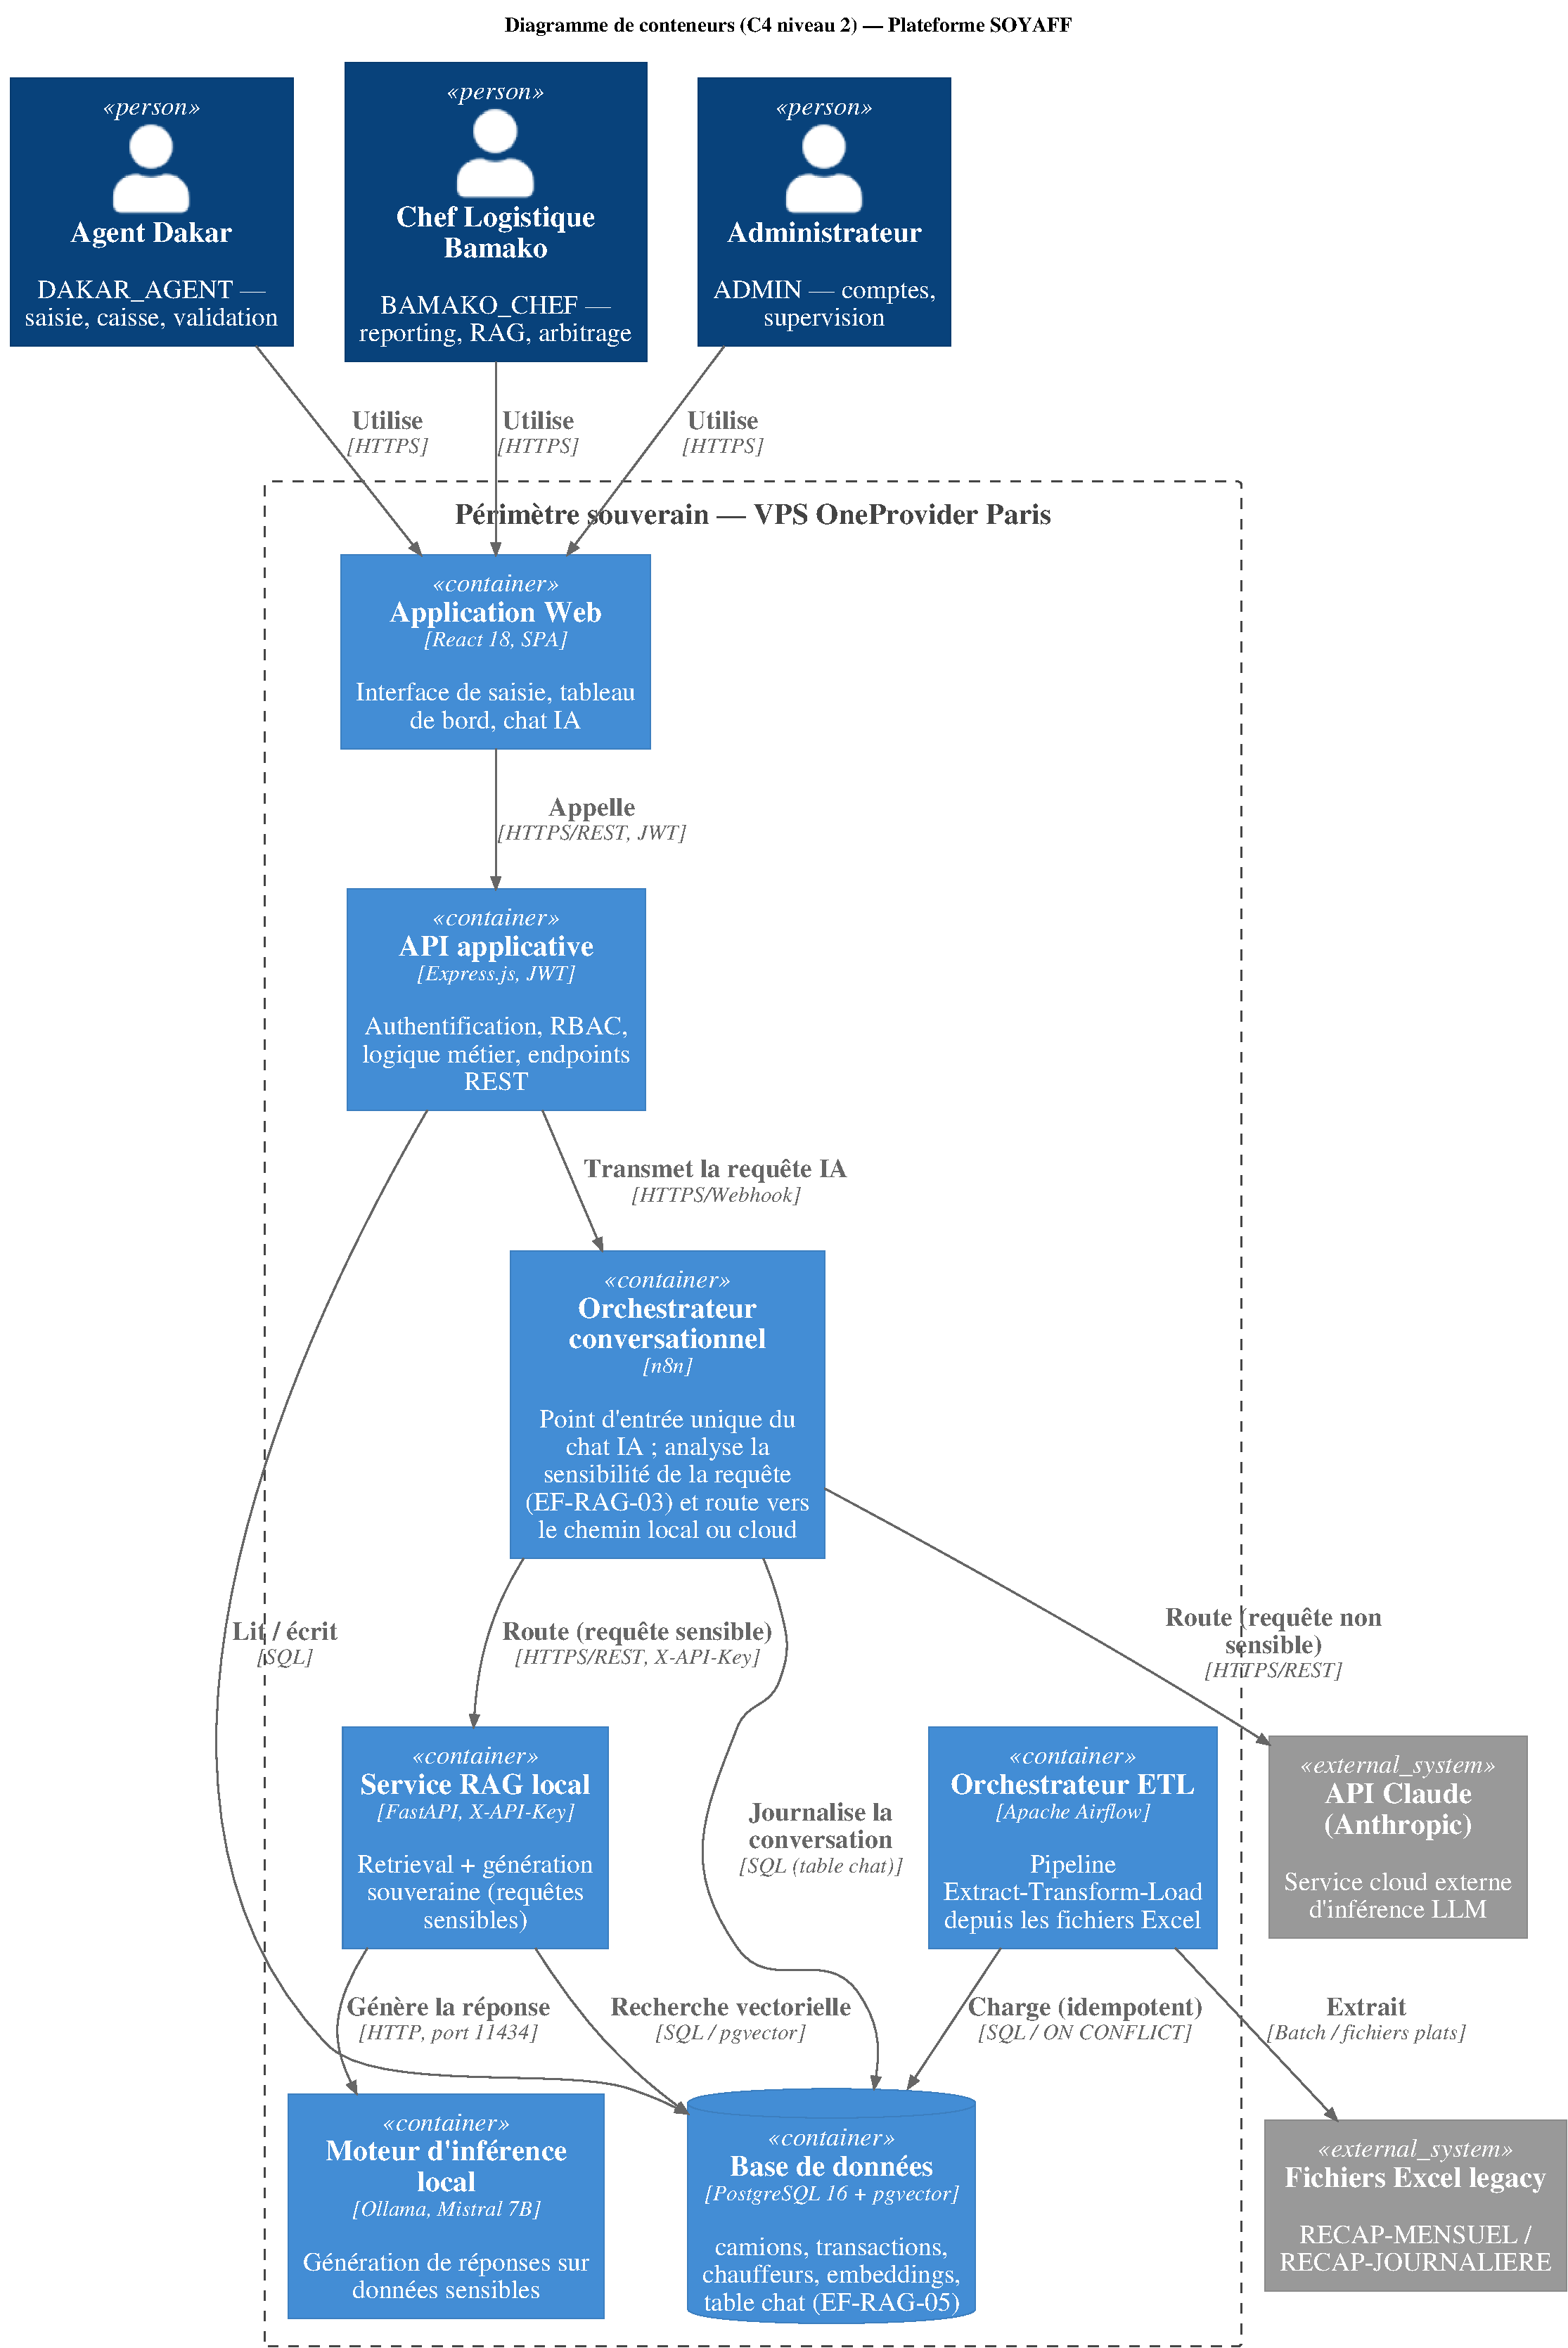
\includegraphics[width=\textwidth,height=0.88\textheight,keepaspectratio]{figures/fig_c4_conteneurs.pdf}
    \caption{Diagramme de conteneurs (C4 niveau 2), plateforme SOYAFF}
    \label{fig:c4_conteneurs}
    \source{Schéma de l'auteur}
\end{figure}

\subsection{Vue de composants : service RAG local}
\label{sec:c4_composants}
Nous ne détaillons le niveau 3 (composants) que pour le conteneur le plus significatif. La Figure~\ref{fig:c4_composants_rag} isole donc les composants internes du service RAG local (FastAPI) : le gestionnaire de requêtes, un composant de réponses SQL directes (comptages, solde), le module de retrieval (filtres SQL puis repli vectoriel \texttt{all-MiniLM-L6-v2}), le constructeur de contexte et le client d'inférence. Les questions de comptage, de solde et de total sont servies sans modèle de langage ; les autres sont confiées à Mistral~7B. Cette vue met aussi en évidence deux écarts à l'exigence de maintenabilité (\texttt{ENF-MAINT-01}, \texttt{ENF-MAINT-02}), détaillés au §\ref{sec:ia_dettes}.

\begin{figure}[H]
    \centering
    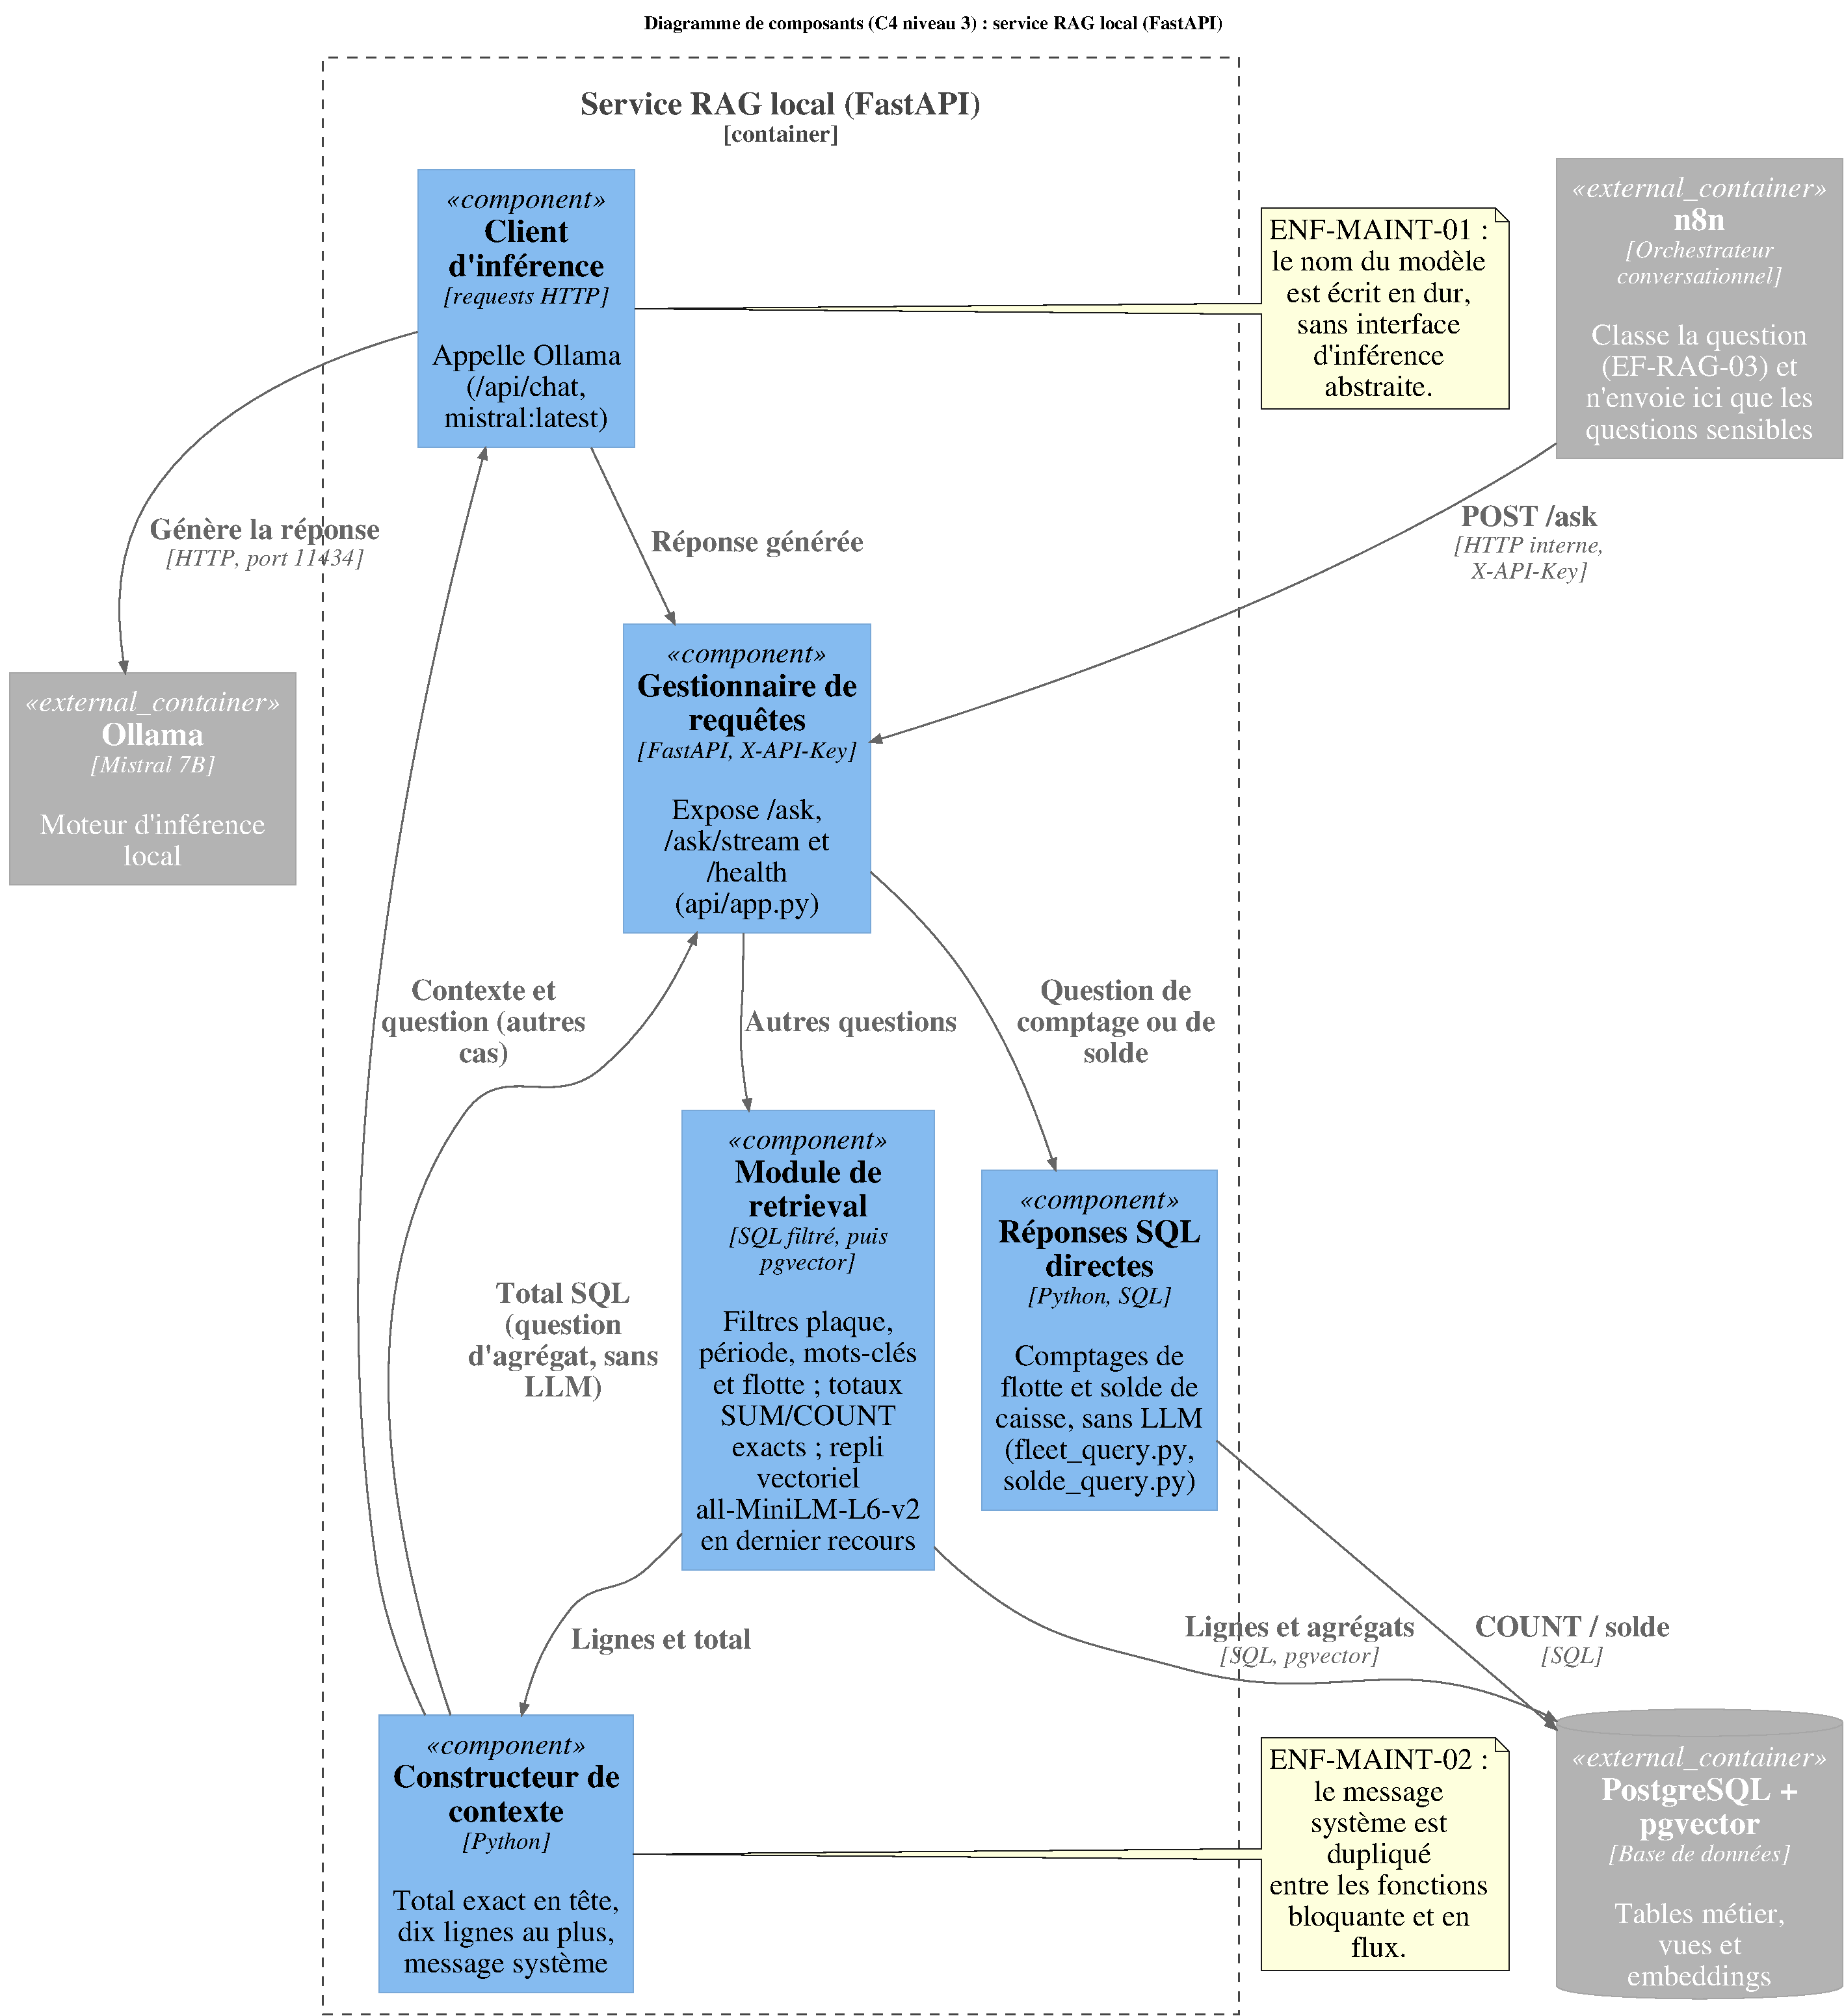
\includegraphics[width=\textwidth,height=0.88\textheight,keepaspectratio]{figures/fig_c4_composants_rag.pdf}
    \caption{Diagramme de composants (C4 niveau 3), service RAG local}
    \label{fig:c4_composants_rag}
    \source{Schéma de l'auteur}
\end{figure}

\subsection{Déploiement}
\label{sec:deploiement}
La Figure~\ref{fig:deploiement} décrit l'infrastructure de production : tous les conteneurs applicatifs, IA, ETL et de supervision sont hébergés sur un seul serveur dédié, ce qui soutient directement l'hypothèse de frugalité H1 (\texttt{ENF-FRUG-01}). Le trafic des clients passe par Cloudflare, chiffré de bout en bout (ADR-05). Quatre services externes complètent le schéma : l'API Anthropic pour le chemin cloud, GitLab.com pour les dépôts et les pipelines, Telegram pour les alertes et l'espace de sauvegarde de l'hébergeur. Pour rester lisible, le schéma est présenté en deux vues : la vue d'ensemble du serveur et de ses flux externes (Figure~\ref{fig:deploiement}), puis le détail des conteneurs du réseau Docker (Figure~\ref{fig:deploiement_docker}).

\begin{landscape}
\begin{figure}[p]
    \centering
    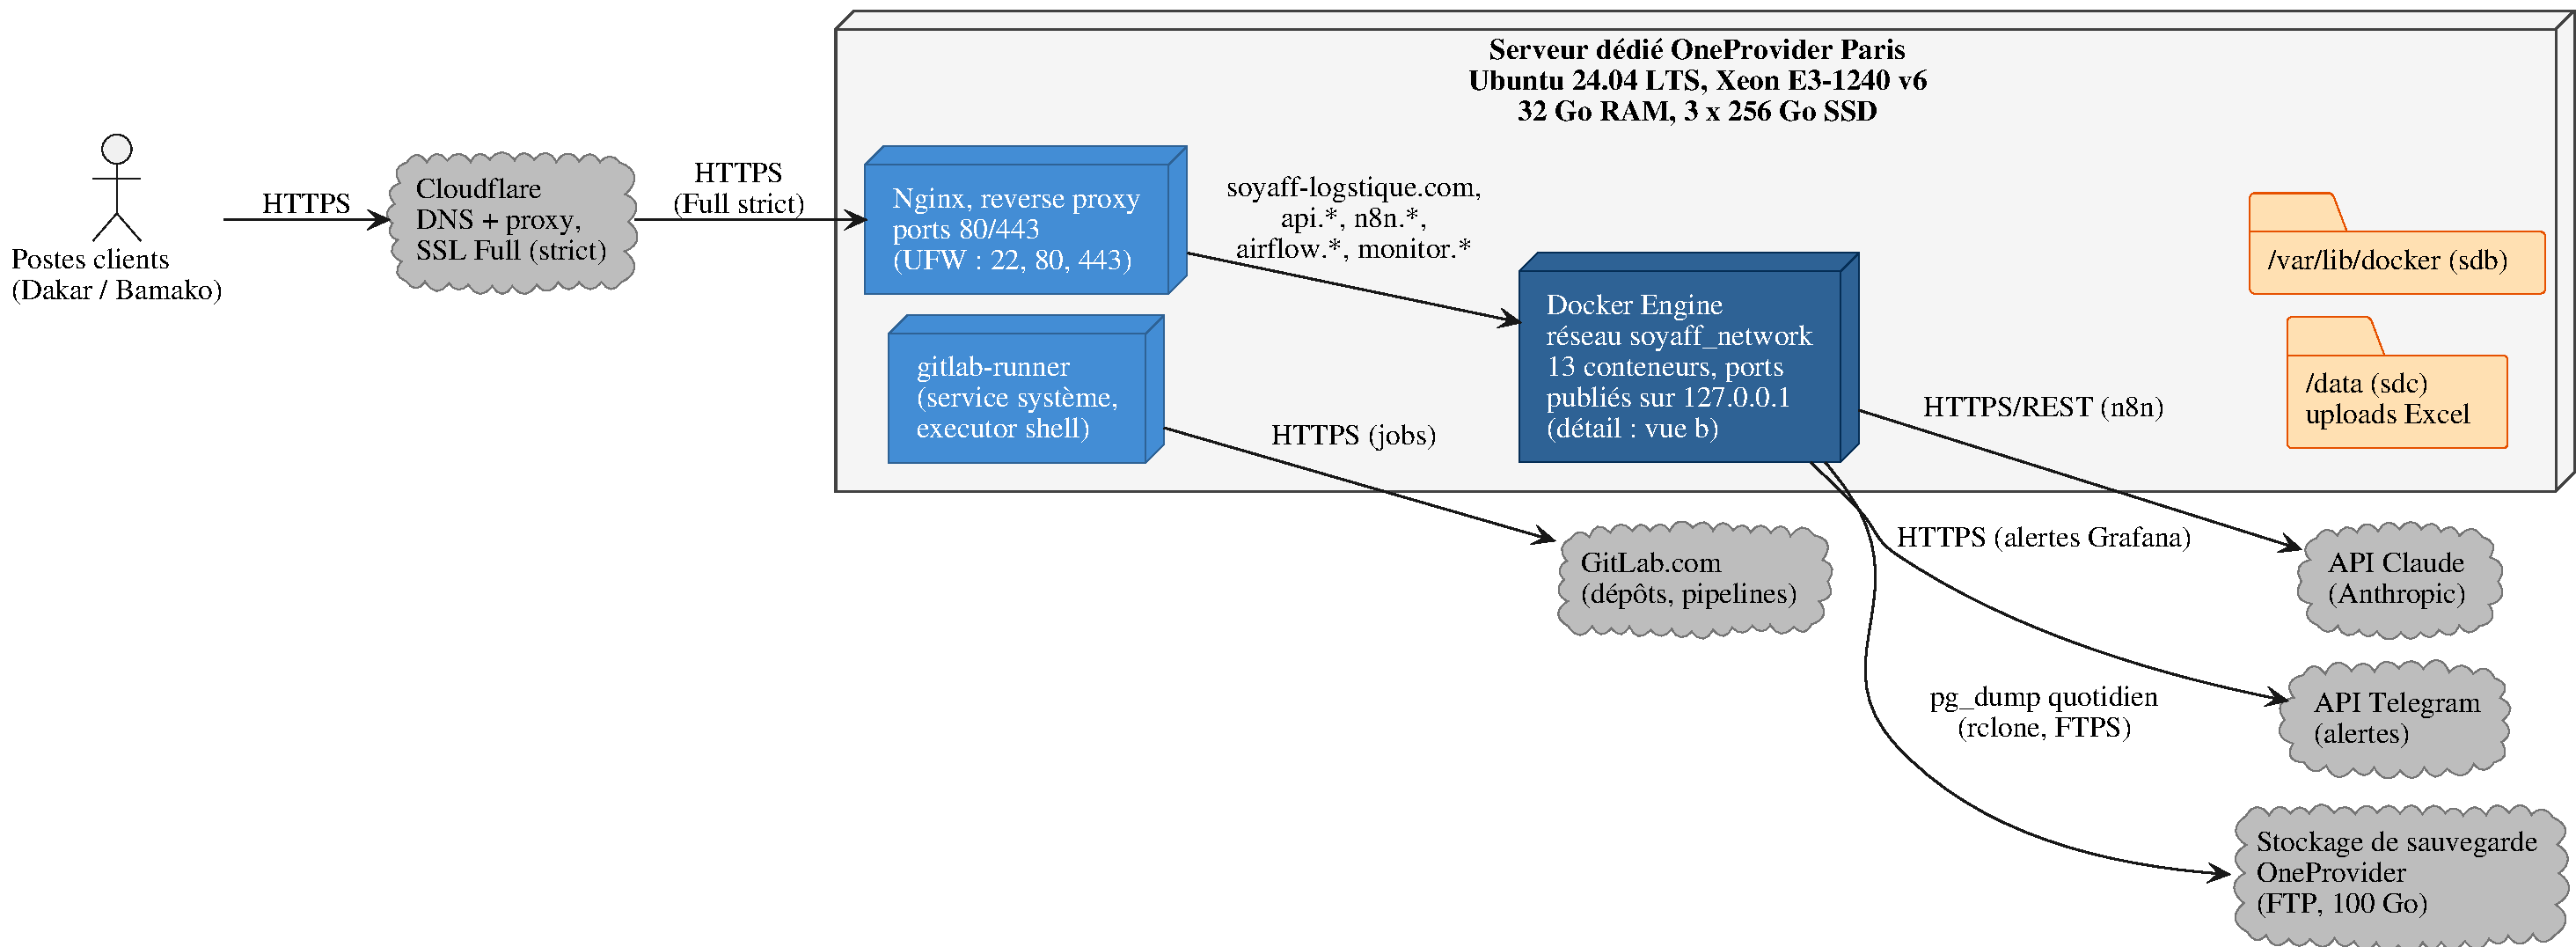
\includegraphics[width=\linewidth,height=0.86\textheight,keepaspectratio]{figures/fig_deploiement_vue.pdf}
    \caption{Diagramme de déploiement (1/2) : serveur de production et services externes}
    \label{fig:deploiement}
    \source{Schéma de l'auteur}
\end{figure}
\begin{figure}[p]
    \centering
    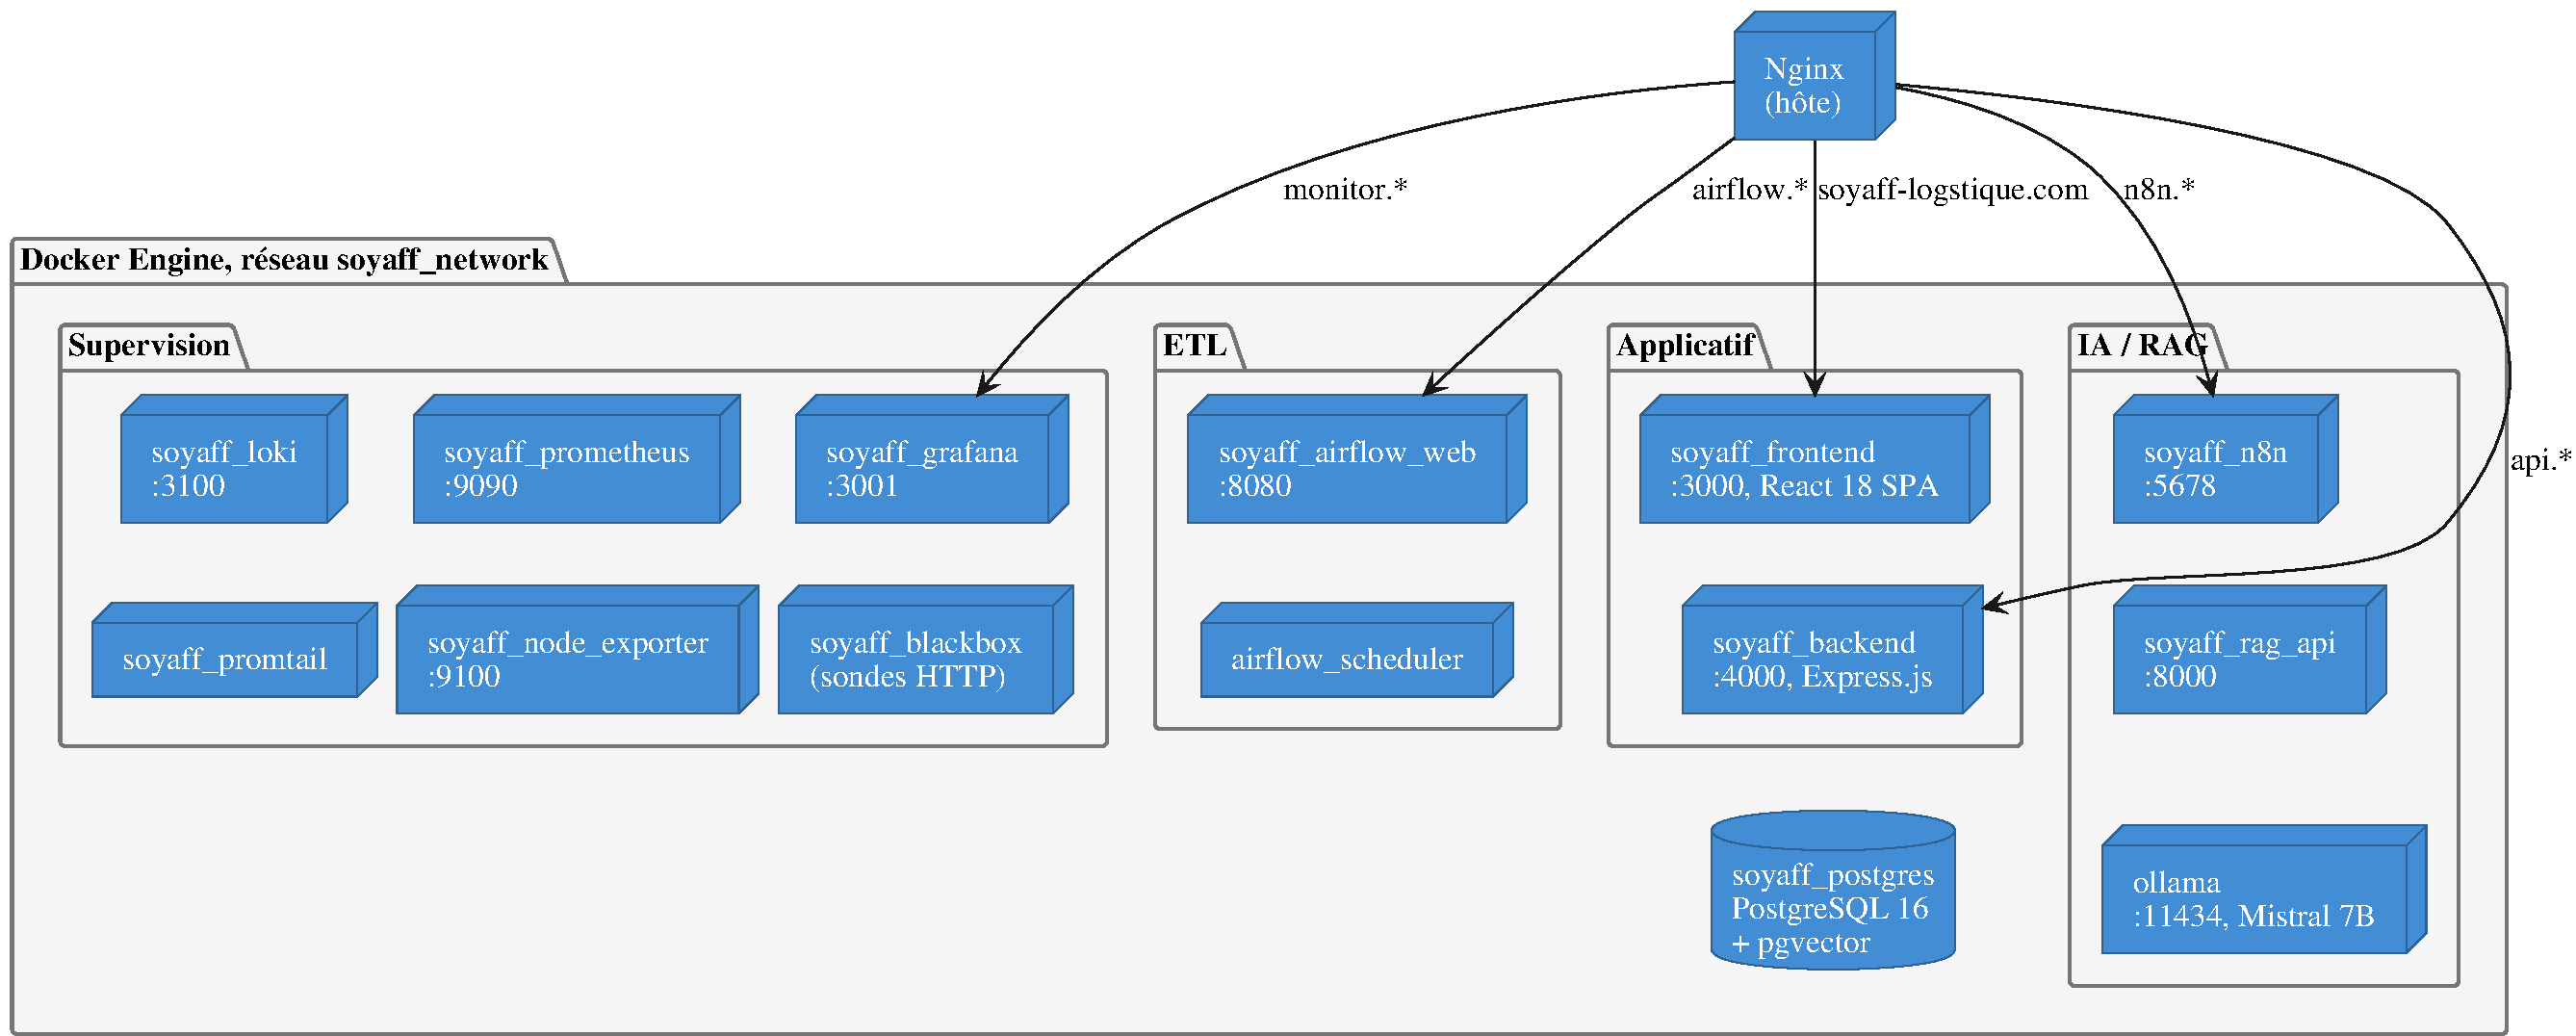
\includegraphics[width=\linewidth,height=0.86\textheight,keepaspectratio]{figures/fig_deploiement_docker.pdf}
    \caption{Diagramme de déploiement (2/2) : conteneurs du réseau Docker \texttt{soyaff\_network}}
    \label{fig:deploiement_docker}
    \source{Schéma de l'auteur}
\end{figure}
\end{landscape}

\subsection{Registre des décisions architecturales (ADR)}
\label{sec:adr}
Les vues précédentes décrivent l'architecture retenue. Cette section en justifie les décisions sous forme d'Architecture Decision Records (ADR) : contexte, option retenue, conséquences (bénéfices comme dettes assumées), et alternatives écartées.

\subsubsection*{ADR-01 : Orchestration ETL par Apache Airflow}
\textbf{Contexte.} Le pipeline d'ingestion des fichiers Excel hétérogènes (\texttt{RECAP-MENSUEL}, \texttt{RECAP-JOURNALIERE}) exige planification, idempotence et gestion de \textit{backfill} en environnement à connectivité intermittente, propre au corridor Dakar--Bamako (§2.2.3). Le choix de l'orchestrateur devait concilier maturité technique et indépendance vis-à-vis des éditeurs commerciaux (§2.2.4).

\textbf{Décision.} Apache Airflow est retenu comme orchestrateur ETL, modélisant le pipeline sous forme de DAG Python idempotents, la déduplication reposant sur la clé \texttt{source\_key} (\texttt{ON CONFLICT DO NOTHING}).

\textbf{Conséquences.} \textit{Positives} : licence Apache~2.0 garantissant une indépendance totale vis-à-vis d'un éditeur ; large éventail de connecteurs matures pour sources hétérogènes (Excel, PDF, PostgreSQL) ; gestion native du \textit{backfill}. \textit{Négatives} : courbe d'apprentissage modérée à difficile ; empreinte ressources plus lourde qu'un ordonnanceur léger de type \textit{cron}.

\textbf{Alternatives écartées.} Prefect et Dagster, tous deux adossés à un modèle commercial cloud qui réintroduirait précisément la dépendance logicielle exogène que l'architecture cherche à éviter (§2.2.4).

\textbf{Exigences / hypothèses liées.} \texttt{EF-ETL-01}, \texttt{EF-ETL-02}, \texttt{ENF-VOL-01}, H4.

\subsubsection*{ADR-02 : Routage hybride cloud/local par sensibilité}
\textbf{Contexte.} Une tension oppose la souveraineté des données sensibles (identités des chauffeurs, montants, opérations financières) à la puissance de calcul disponible localement pour l'inférence LLM, le serveur ne disposant d'aucun GPU dédié (§2.4). Le besoin décisionnel exprimé par \texttt{EF-RAG-01/02} exige néanmoins un agent conversationnel capable de traiter des requêtes analytiques complexes.

\textbf{Décision.} La sensibilité de chaque requête est classifiée en amont par un nœud d'analyse par mots-clés au sein du workflow n8n, qui route ensuite vers l'un de deux chemins : le service RAG local (FastAPI + pgvector + Ollama/Mistral, aucune sortie réseau) pour les requêtes sensibles, l'API Claude cloud pour les requêtes non sensibles.

\textbf{Conséquences.} \textit{Positives} : conformité déclarative à \texttt{ENF-SOUV-01} pour le périmètre classé sensible ; accès à la puissance d'un LLM cloud pour les requêtes complexes sans investissement GPU. \textit{Négatives} : la classification par mots-clés reste une heuristique et non un mécanisme certifié, avec un risque résiduel de faux négatif (requête sensible mal classée et routée vers le cloud) ; le chemin local ne repose pas encore sur une interface d'inférence abstraite (écart \texttt{ENF-MAINT-01}, §\ref{sec:c4_composants}). \textit{Résolu} (section~\ref{chap:ia_rag}, §\ref{sec:ia_routage}) : le workflow n8n est versionné et le routage a été vérifié dans les deux sens ; une mention d'identité (chauffeur, plaque) reste désormais locale même dans une question d'agrégat ; l'outil SQL de l'agent cloud utilise un rôle PostgreSQL en lecture seule, sans accès aux données des chauffeurs.

\textbf{Alternatives écartées.} Tout-cloud, écarté comme incompatible avec \texttt{ENF-SOUV-01} et H2 ; tout-local, écarté faute de puissance suffisante pour satisfaire \texttt{ENF-PERF-02/03} sur les requêtes analytiques complexes avec le matériel disponible.

\textbf{Exigences / hypothèses liées.} \texttt{EF-RAG-01} à \texttt{05}, \texttt{ENF-SOUV-01}, \texttt{ENF-SOUV-02}, H2.

\subsubsection*{ADR-03 : Déploiement mono-hôte sur serveur dédié unique}
\textbf{Contexte.} La contrainte budgétaire d'une PME subsaharienne (H1) doit être mise en balance avec le nombre croissant de services nécessaires à la plateforme (applicatif, IA, ETL, observabilité, CI/CD).

\textbf{Décision.} L'intégralité de la plateforme (quatorze conteneurs Docker) est hébergée sur un unique serveur dédié (OneProvider Paris, Xeon E3-1240 v6, 32~Go RAM, 3~$\times$~256~Go SSD), orchestrés via Docker Engine sur un réseau applicatif unique (\texttt{soyaff\_network}).

\textbf{Conséquences.} \textit{Positives} : coût d'infrastructure minimal, compatible avec \texttt{ENF-FRUG-01} ; simplicité opérationnelle d'un point d'administration unique. \textit{Négatives} : point de défaillance unique (\textit{SPOF}), donc aucune haute disponibilité : une panne matérielle ou une saturation de ressource affecte simultanément l'ensemble des services ; absence de scalabilité horizontale native. Cette dette est assumée explicitement et reprise à la section~\ref{chap:discussion}.

\textbf{Alternatives écartées.} Déploiement multi-nœuds ou infrastructure managée (Kubernetes cloud, bases de données managées), au coût mensuel incompatible avec \texttt{ENF-FRUG-01} et la réalité budgétaire d'une PME du secteur.

\textbf{Exigences / hypothèses liées.} \texttt{ENF-FRUG-01}, \texttt{ENF-DISP-02}, H1.

\subsubsection*{ADR-04 : PostgreSQL + pgvector plutôt qu'une base vectorielle dédiée}
\textbf{Contexte.} Le RAG local requiert un stockage d'embeddings vectoriels pour la recherche par similarité, en complément du stockage relationnel déjà nécessaire aux données métier (transactions, camions, chauffeurs).

\textbf{Décision.} Le stockage relationnel et vectoriel est mutualisé au sein d'un unique moteur PostgreSQL~16 étendu par \texttt{pgvector}, plutôt que de déployer une base vectorielle dédiée.

\textbf{Conséquences.} \textit{Positives} : un conteneur de moins à opérer et sécuriser, cohérent avec l'ADR-03 ; cohérence transactionnelle native entre données métier et embeddings, source de vérité unique facilitant la sauvegarde (\texttt{EF-ADM-03}) ; requêtes hybrides SQL/vectorielles en une seule transaction. \textit{Négatives} : performances de recherche vectorielle a priori inférieures à celles d'une base spécialisée sur de très gros volumes, ce qui n'est pas discriminant à la volumétrie actuelle de SOYAFF (\texttt{ENF-VOL-02}).

\textbf{Alternatives écartées.} Pinecone, écarté comme service SaaS propriétaire incompatible avec la souveraineté visée par H2 ; Qdrant ou Weaviate en conteneur dédié, fonctionnellement solides mais ajoutant un service supplémentaire à opérer sans bénéfice mesurable au volume actuel, à rebours de la frugalité visée par H1.

\textbf{Exigences / hypothèses liées.} \texttt{ENF-FRUG-01}, \texttt{ENF-SOUV-01}, \texttt{ENF-VOL-02}.

\subsubsection*{ADR-05 : Terminaison TLS Cloudflare (« Flexible », révisée en « Full (strict) »)}
\textbf{Contexte.} La mise en production rapide de la plateforme devait garantir un chiffrement du trafic client sans mobiliser de temps d'ingénierie supplémentaire pour la gestion de certificats sur le serveur.

\textbf{Décision.} Le mode SSL «\,Flexible\,» de Cloudflare avait d'abord été activé : il chiffrait le trajet poste client~$\rightarrow$~Cloudflare, mais laissait le trajet Cloudflare~$\rightarrow$~origine (serveur) en HTTP.

\textbf{Conséquences.} \textit{Positive} : mise en place immédiate, sans gestion de certificat côté serveur. \textit{Négative} : le trajet Cloudflare~$\rightarrow$~origine restait en clair, ce qui constituait un écart non conforme à \texttt{ENF-SEC-05} (chiffrement de bout en bout). Cette configuration a été traitée comme une dette technique assumée plutôt que comme un choix définitif.

\textbf{Alternatives écartées.} Mode Cloudflare «\,Full (strict)\,» avec certificat installé sur le serveur, écarté au départ pour des raisons de délai de mise en production.

\textbf{Révision (26~septembre~2026).} Le mode «\,Full (strict)\,» est désormais actif : le trajet Cloudflare~$\rightarrow$~origine est chiffré et le certificat du serveur est vérifié (§\ref{sec:devops_securite}). L'écart à \texttt{ENF-SEC-05} est refermé.

\textbf{Exigences / hypothèses liées.} \texttt{ENF-SEC-05}.

Cette section a posé l'architecture : quatre vues C4 et cinq décisions structurantes tracées en ADR, qui referment la conception ouverte par l'analyse des besoins. Chaque choix reste relié à une exigence, et in fine à une hypothèse de recherche. Les écarts entre conception et implémentation (interface d'inférence non abstraite, par exemple) sont des dettes assumées, reprises à la section~\ref{chap:discussion}. La Partie~III traduit maintenant ce plan en système opérationnel : pipeline d'ingestion, application web, module d'IA, infrastructure DevOps.

